\documentclass{article}%
\usepackage[T1]{fontenc}%
\usepackage[utf8]{inputenc}%
\usepackage{lmodern}%
\usepackage{textcomp}%
\usepackage{lastpage}%
%
\usepackage{amsmath}%
\usepackage{amssymb}%
\usepackage{amsfonts}%
\usepackage{graphicx}%
\usepackage{hyperref}%
\usepackage{tikz}%
\usepackage{pgfplots}%
\usetikzlibrary{math}%
\title{ITA 2027 - Química\thanks{This exam was solved and automatically generated with gpt-resolve: \url{https://github.com/lgabs/gpt-resolve}}}%
\author{claude{-}sonnet{-}5{-}5 (solver) + claude{-}sonnet{-}5{-}5 (judge)}%
\date{November 09, 2026}%
%
\begin{document}%
\normalsize%
\maketitle%
\section*{Questão 1}

\section*{Solução}

\textbf{Hipóteses.} Gases ideais; combustão completa; todo o calor liberado vai para os gases produzidos e os que não reagiram (processo isobárico, $Q_p=\Delta H$); $C_p=40\ \mathrm{J\,K^{-1}\,mol^{-1}}$ constante e igual para qualquer composição da mistura; a água permanece como vapor (ela faz parte da mistura gasosa citada no enunciado).

\subsection*{a) Equação balanceada}
\[
\mathrm{C_5H_{12}(g)} + 8\,\mathrm{O_2(g)} \longrightarrow 5\,\mathrm{CO_2(g)} + 6\,\mathrm{H_2O(g)},\qquad \Delta H_c=-3440\ \mathrm{kJ\,mol^{-1}} .
\]
(Balanceamento: 5 C $\to$ 5 CO$_2$; 12 H $\to$ 6 H$_2$O; O: $10+6=16$ $\to$ 8 O$_2$.)

\subsection*{b) Quantidades de O$_2$ e N$_2$}
Quantidade total de ar admitido, com $P=1\ \mathrm{bar}=10^{5}\ \mathrm{Pa}$, $V=200\ \mathrm{L}=0{,}200\ \mathrm{m^3}$ e $T=300{,}84\ \mathrm{K}$:
\[
n_{ar}=\frac{PV}{RT}=\frac{10^{5}\cdot 0{,}200}{8{,}31\cdot 300{,}84}=\frac{20000}{2500}=8{,}0\ \mathrm{mol}.
\]
(Com $R=0{,}0821\ \mathrm{atm\,L\,K^{-1}\,mol^{-1}}$ e $1\ \mathrm{bar}=0{,}987\ \mathrm{atm}$ obtém-se $7{,}99\approx 8{,}0$ mol.) Então:
\[
n_{\mathrm{O_2}}=0{,}20\cdot 8{,}0=\mathbf{1{,}6\ mol},\qquad n_{\mathrm{N_2}}=0{,}80\cdot 8{,}0=\mathbf{6{,}4\ mol}.
\]

\subsection*{c) Temperatura na condição estequiométrica}
Todo o O$_2$ é consumido: $n_{\mathrm{C_5H_{12}}}=1{,}6/8=0{,}20$ mol. Calor liberado:
\[
Q=0{,}20\cdot 3440\ \mathrm{kJ}=688\ \mathrm{kJ}.
\]
Gases finais: N$_2$ $=6{,}4$ mol; CO$_2$ $=5(0{,}20)=1{,}0$ mol; H$_2$O $=6(0{,}20)=1{,}2$ mol; total $n_f=8{,}6$ mol (sobra O$_2$ nulo). Balanço de energia (calor da reação aquecendo os produtos):
\[
Q=n_f\,C_p\,\Delta T\ \Rightarrow\ \Delta T=\frac{688\,000}{8{,}6\cdot 40}=\frac{688\,000}{344}=2000\ \mathrm{K}
\]
\[
T_f=300{,}84+2000=\mathbf{2300{,}84\ K}.
\]

\subsection*{d) Quantidade de combustível para $T_f=1600{,}84$ K}
Agora $\Delta T=1600{,}84-300{,}84=1300$ K. Como a temperatura máxima ($2300{,}84$ K) ocorre na condição estequiométrica, $1600{,}84$ K só é atingida com mistura \emph{pobre} (falta de combustível, excesso de O$_2$) ou \emph{rica} (excesso de combustível). A condição de \textbf{economia de combustível} escolhe a mistura pobre (a rica exigiria cerca de $4{,}6$ mol de pentano não queimado, desperdício enorme e combustão incompleta, contrariando o enunciado).

Seja $x<0{,}20$ mol de pentano queimado (completamente, pois há O$_2$ em excesso). Gases finais:
\[
\mathrm{O_2}:\ 1{,}6-8x;\quad \mathrm{N_2}:\ 6{,}4;\quad \mathrm{CO_2}:\ 5x;\quad \mathrm{H_2O}:\ 6x
\ \Rightarrow\ n_f=8{,}0+3x .
\]
Balanço de energia:
\[
3440\,000\,x=40\,(8{,}0+3x)\cdot 1300=416\,000+156\,000\,x
\]
\[
x=\frac{416\,000}{3\,284\,000}=0{,}1267\ \mathrm{mol}.
\]
Em relação ao estequiométrico:
\[
\frac{x}{0{,}20}=0{,}633\approx 63\%\ ,
\]
isto é, o combustível deve ser \textbf{reduzido em $\approx 37\%$} (usar $\approx 63\%$ da quantidade estequiométrica).

\textbf{Verificação:} $Q=3440\cdot0{,}1267=435{,}8$ kJ; $n_f=8{,}380$ mol; $\Delta T=435\,800/(40\cdot 8{,}380)=1300$ K $\checkmark$. Ordem de grandeza coerente: menos combustível $\Rightarrow$ menos calor e $T$ menor que $2300{,}84$ K; o O$_2$ residual ($1{,}6-1{,}01=0{,}59$ mol) confirma a mistura pobre.

ANSWER: a) $\mathrm{C_5H_{12}+8\,O_2\to5\,CO_2+6\,H_2O}$; b) $n_{\mathrm{O_2}}=1{,}6$ mol e $n_{\mathrm{N_2}}=6{,}4$ mol; c) $T=2300{,}84$ K; d) reduzir o combustível em $\approx 37\%$ (usar $\approx 63\%$ da quantidade estequiométrica, $\approx 0{,}127$ mol de pentano).%
\newpage%
\section*{Questão 2}

\section*{Solução}
\pgfplotsset{compat=1.14}

\textbf{1. Dados e hipóteses.} Volume inicial da solução: $V_0=A\,h=1\ \text{dm}^2\times 10\ \text{dm}=10\ \text{dm}^3=10\ \text{L}$. A massa de soluto é $m=0{,}2\times 80=16$ g, logo $c_0=\dfrac{0{,}2\ \text{mol}}{10\ \text{L}}=0{,}020\ \text{mol/L}=1{,}6\ \text{g/L}$. A solubilidade é $4\ \text{g/L}=\dfrac{4}{80}=0{,}050\ \text{mol/L}$. Como $1{,}6<4$ g/L, todo o soluto está inicialmente dissolvido.

Hipóteses: soluto molecular (não eletrólito, $i=1$) e solução diluída ideal, de modo que vale a lei de van't Hoff, $\pi=cRT$. A membrana só deixa passar solvente. O solvente é incompressível e o volume do soluto é desprezível. Como a compressão é reversível, a pressão aplicada é $P_{atm}+\pi$, em que $\pi$ é a pressão osmótica \emph{instantânea} da solução, que varia ao longo do processo.

\textbf{2. Relação entre o deslocamento e o volume.} Se o êmbolo desce $x$ dm, passam para o compartimento do solvente $A\,x=x$ L de solvente. O soluto permanece, então
\[
V(x)=(10-x)\ \text{L},\qquad c(x)=\frac{n}{V}=\frac{0{,}2}{10-x}\ \text{mol/L},
\]
enquanto a solução não estiver saturada. O êmbolo do solvente sobe, mas o solvente puro continua sob $P_{atm}$, o que não altera $\pi$.

Com $RT=0{,}0821\times 305=25{,}04\ \text{atm}\cdot\text{L}\cdot\text{mol}^{-1}$:

\textbf{3. Região I (solução insaturada).} Para $0\le x\le x_s$,
\[
\pi(x)=c\,RT=\frac{0{,}2\times 25{,}04}{10-x}=\frac{5{,}008}{10-x}\ \text{atm}.
\]
Em $x=0$: $\pi_0=0{,}020\times 25{,}04\approx 0{,}50$ atm.

\textbf{4. Início da saturação.} A saturação ocorre quando $c=0{,}050$ mol/L:
\[
\frac{0{,}2}{10-x_s}=0{,}050\ \Rightarrow\ 10-x_s=4\ \text{L}\ \Rightarrow\ x_s=6\ \text{dm},\qquad
\pi_s=0{,}050\times 25{,}04\approx 1{,}25\ \text{atm}.
\]

\textbf{5. Região II (solução saturada).} Para $6\le x\le 9$ dm, o soluto em excesso precipita e fica retido, pois a membrana não o deixa passar. A solução permanece saturada, com $c=0{,}050$ mol/L constante, então
\[
\pi=0{,}050\times 25{,}04\approx 1{,}25\ \text{atm (constante)}.
\]
Em $x=9$ dm, $V=1$ L dissolve $0{,}05$ mol (4 g), e $0{,}15$ mol (12 g) estão precipitados. Sem a precipitação, $\pi\to\infty$ quando $x\to 10$ dm, o que seria fisicamente absurdo.

\textbf{6. Valores e gráfico.}
\begin{center}
\begin{tabular}{c|ccccccccccc}
$x$ (dm) & 0 & 1 & 2 & 3 & 4 & 5 & 6 & 7 & 8 & 9\\ \hline
$V$ (L) & 10 & 9 & 8 & 7 & 6 & 5 & 4 & 3 & 2 & 1\\
$\pi$ (atm) & 0,50 & 0,56 & 0,63 & 0,72 & 0,83 & 1,00 & 1,25 & 1,25 & 1,25 & 1,25
\end{tabular}
\end{center}

\begin{center}
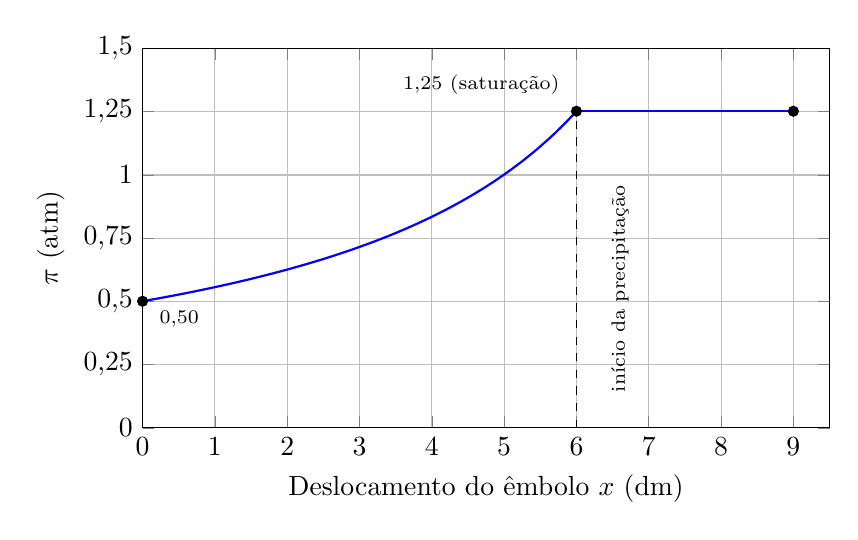
\begin{tikzpicture}
\begin{axis}[width=0.85\linewidth,height=6.4cm,
 xlabel={Deslocamento do êmbolo $x$ (dm)},ylabel={$\pi$ (atm)},
 xmin=0,xmax=9.5,ymin=0,ymax=1.5,xtick={0,1,...,9},ytick={0,0.25,...,1.5},
 grid=both,minor tick num=0,
 yticklabel style={/pgf/number format/.cd,fixed,precision=2,use comma}]
\addplot[domain=0:6,samples=61,thick,blue]{5.0081/(10-x)};
\addplot[thick,blue] coordinates {(6,1.252) (9,1.252)};
\addplot[only marks,mark=*,mark size=1.8pt,black] coordinates {(0,0.5008)(6,1.252)(9,1.252)};
\draw[dashed] (axis cs:6,0) -- (axis cs:6,1.252);
\node[anchor=north west,font=\scriptsize] at (axis cs:0.1,0.5008) {0,50};
\node[anchor=south east,font=\scriptsize] at (axis cs:5.9,1.28) {1,25 (saturação)};
\node[anchor=north,font=\scriptsize,rotate=90] at (axis cs:6.35,0.55) {início da precipitação};
\end{axis}
\end{tikzpicture}
\end{center}

O gráfico é um ramo de hipérbole, $\pi=5{,}008/(10-x)$, de $0{,}50$ atm em $x=0$ até $1{,}25$ atm em $x=6$ dm, seguido de um patamar horizontal em $1{,}25$ atm até $x=9$ dm.

\textbf{7. Conferência.} A unidade de $cRT$ é $\text{mol/L}\cdot\text{atm}\,\text{L}\,\text{mol}^{-1}\text{K}^{-1}\cdot\text{K}=\text{atm}$. A curva é contínua em $x=6$ dm, com $\pi$ crescente e proporcional a $1/V$. A ordem de grandeza está coerente, pois $0{,}02$ mol/L dá cerca de $0{,}5$ atm ($1$ mol/L daria cerca de $25$ atm). Aumentar $c$ em $2{,}5$ vezes, de $0{,}02$ para $0{,}05$ mol/L, aumenta $\pi$ na mesma razão, de $0{,}50$ para $1{,}25$ atm.

ANSWER: $\pi(x)=\dfrac{5{,}008}{10-x}$ atm para $0\le x\le 6$ dm (de $0{,}50$ a $1{,}25$ atm; hipérbole) e $\pi=1{,}25$ atm constante para $6\le x\le 9$ dm (solução saturada, soluto precipitando).%
\newpage%
\section*{Questão 3}

\section*{Solução}

\textbf{Passo 1 --- Item (a): desidratação do álcool (X).}
O 2-metilbutan-2-ol é um álcool terciário. Com $\mathrm{H_2SO_4}$ e aquecimento ocorre desidratação intramolecular (eliminação E1): protonação da hidroxila, saída de $\mathrm{H_2O}$ com formação do carbocátion terciário $\mathrm{(CH_3)_2C^{+}CH_2CH_3}$ e perda de um $\mathrm{H^+}$ de um carbono vizinho. Há dois $\beta$-hidrogênios possíveis: nos grupos $\mathrm{CH_3}$ (dá o alceno 2-metilbut-1-eno, dissubstituído) e no $\mathrm{CH_2}$ (dá o 2-metilbut-2-eno, trissubstituído). Pela regra de Zaitsev, predomina o alceno mais substituído (mais estável):
\[
\boxed{\mathrm{X:\ (CH_3)_2C{=}CH{-}CH_3}}\qquad\text{(2-metilbut-2-eno)}
\]
(o 2-metilbut-1-eno é apenas o produto minoritário).

\textbf{Passo 2 --- Item (b): adição de HBr sem peróxido (Z).}
Sem peróxido a adição é eletrofílica e iônica, seguindo a regra de Markovnikov. O $\mathrm{H^+}$ liga-se ao carbono sp$^2$ que já tem hidrogênio ($\mathrm{C}_3$), pois isso gera o carbocátion mais estável, o terciário em $\mathrm{C}_2$. Em seguida $\mathrm{Br^-}$ ataca esse carbocátion:
\[
\mathrm{(CH_3)_2C{=}CH{-}CH_3 + HBr \longrightarrow (CH_3)_2C(Br){-}CH_2{-}CH_3}
\]
\[
\boxed{\mathrm{Z:\ (CH_3)_2CBr{-}CH_2CH_3}}\qquad\text{(2-bromo-2-metilbutano)}
\]

\textbf{Passo 3 --- Item (c): adição de HBr com peróxido (G).}
Na presença de peróxido a adição é radicalar (efeito Kharasch, anti-Markovnikov):
\begin{itemize}
\item iniciação: $\mathrm{RO{-}OR \to 2\,RO^{\bullet}}$ e $\mathrm{RO^{\bullet} + HBr \to ROH + Br^{\bullet}}$;
\item propagação 1: $\mathrm{Br^{\bullet}}$ ataca o carbono sp$^2$ menos impedido ($\mathrm{C}_3$), formando o radical terciário, mais estável, em $\mathrm{C}_2$: $\mathrm{(CH_3)_2C^{\bullet}{-}CHBr{-}CH_3}$;
\item propagação 2: esse radical abstrai $\mathrm{H^{\bullet}}$ de outra molécula de HBr, formando o produto e regenerando $\mathrm{Br^{\bullet}}$.
\end{itemize}
O Br fica no carbono menos substituído e o H no mais substituído, o inverso do item (b):
\[
\boxed{\mathrm{G:\ (CH_3)_2CH{-}CHBr{-}CH_3}}\qquad\text{(2-bromo-3-metilbutano)}
\]
O $\mathrm{C}_2$ de G (o $\mathrm{CHBr}$) é estereocentro, mas, sem reagente quiral, forma-se a mistura racêmica.

\textbf{Passo 4 --- Item (d): $\mathrm{KMnO_4}$ diluído, $\mathrm{OH^-}$, a frio (J).}
Essas condições (permanganato diluído, meio básico, baixa temperatura) fazem di-hidroxilação \emph{sin} da dupla (Baeyer): forma-se um éster cíclico de manganato (adição concertada dos dois O pela mesma face), hidrolisado a diol vicinal, e o $\mathrm{Mn(VII)}$ reduz-se a $\mathrm{MnO_2}$ (precipitado marrom). Não há clivagem da ligação C--C, o que exigiria condições drásticas (a quente, concentrado ou ácido):
\[
\mathrm{(CH_3)_2C{=}CH{-}CH_3 \xrightarrow[\ \text{a frio}\ ]{KMnO_4\,(dil.),\ OH^-} (CH_3)_2C(OH){-}CH(OH){-}CH_3}
\]
\[
\boxed{\mathrm{J:\ (CH_3)_2C(OH){-}CH(OH){-}CH_3}}\qquad\text{(2-metilbutano-2,3-diol)}
\]
Só o $\mathrm{C}_3$ é estereocentro (o $\mathrm{C}_2$ tem dois $\mathrm{CH_3}$), então não há diastereoisômeros e J forma-se como par racêmico.

\textbf{Conferência.} X é $\mathrm{C_5H_{10}}$ e os demais produtos conservam o esqueleto de 5 carbonos. Z e G são isômeros, $\mathrm{C_5H_{11}Br}$, com regioquímicas opostas. J é $\mathrm{C_5H_{12}O_2}$ (X mais dois grupos OH). X é o isômero de Zaitsev, o de maior estabilidade.

\medskip
\noindent ANSWER:\\
X $=\mathrm{(CH_3)_2C{=}CHCH_3}$ (2-metilbut-2-eno);\\
Z $=\mathrm{(CH_3)_2CBrCH_2CH_3}$ (2-bromo-2-metilbutano);\\
G $=\mathrm{(CH_3)_2CHCHBrCH_3}$ (2-bromo-3-metilbutano);\\
J $=\mathrm{(CH_3)_2C(OH)CH(OH)CH_3}$ (2-metilbutano-2,3-diol).%
\newpage%
\section*{Questão 4}

\section*{Solução}

\textbf{Hipóteses.} Os sais se dissolvem e dissociam totalmente em água; as impurezas não fornecem os cátions $\mathrm{Q^+}$, $\mathrm{R^{2+}}$, $\mathrm{T^{3+}}$ nem o ânion $\mathrm{X^-}$; o volume final da solução é $V=500\ \mathrm{mL}=0{,}5\ \mathrm{L}$.

\textbf{Passo 1 --- quantidade de cada cátion.} A quantidade total de cátions é
\[
n_{\text{cát}} = C\,V = 2\ \mathrm{mol\cdot L^{-1}}\times 0{,}5\ \mathrm{L} = 1{,}0\ \mathrm{mol}.
\]
Como $\mathrm{Q}:\mathrm{R}:\mathrm{T}=6:3:1$ (soma $=10$ partes), cada parte vale $0{,}10$ mol. Então
\[
n_{\mathrm{Q^+}}=0{,}6\ \mathrm{mol},\qquad n_{\mathrm{R^{2+}}}=0{,}3\ \mathrm{mol},\qquad n_{\mathrm{T^{3+}}}=0{,}1\ \mathrm{mol}.
\]
Cada fórmula (QX, $\mathrm{RX_2}$, $\mathrm{TX_3}$) contém um único cátion, logo $n_{\text{sal puro}}=n_{\text{cátion}}$ (estequiometria 1:1).

\textbf{a) Massa de QX.} Massa de QX puro necessária:
\[
m_{\text{puro}} = 0{,}6\ \mathrm{mol}\times 60\ \mathrm{g\cdot mol^{-1}} = 36\ \mathrm{g}.
\]
Como o sal tem pureza de $90\%$, $0{,}90\,m = 36\ \mathrm{g}$, e portanto
\[
m=\frac{36}{0{,}90}=40\ \mathrm{g}.
\]

\textbf{b) Pureza de $\mathrm{RX_2}$.} Massa de $\mathrm{RX_2}$ puro necessária:
\[
m_{\text{puro}} = 0{,}3\ \mathrm{mol}\times 150\ \mathrm{g\cdot mol^{-1}} = 45\ \mathrm{g}.
\]
Foram pesados $60$ g do sal impuro, então
\[
P=\frac{45}{60}\times 100\% = 75\%.
\]

\textbf{c) Massa molar de $\mathrm{TX_3}$.} Massa de $\mathrm{TX_3}$ puro nos $20$ g pesados:
\[
m_{\text{puro}}=0{,}90\times 20\ \mathrm{g}=18\ \mathrm{g}.
\]
Essa massa corresponde a $0{,}1$ mol, portanto
\[
MM=\frac{18\ \mathrm{g}}{0{,}1\ \mathrm{mol}}=180\ \mathrm{g\cdot mol^{-1}}.
\]

\textbf{d) Concentração de $\mathrm{X^-}$.} Cada mol de QX, $\mathrm{RX_2}$ e $\mathrm{TX_3}$ libera, respectivamente, $1$, $2$ e $3$ mol de $\mathrm{X^-}$:
\[
n_{\mathrm{X^-}} = 1(0{,}6)+2(0{,}3)+3(0{,}1)=0{,}6+0{,}6+0{,}3=1{,}5\ \mathrm{mol},
\]
\[
[\mathrm{X^-}]=\frac{1{,}5\ \mathrm{mol}}{0{,}5\ \mathrm{L}}=3{,}0\ \mathrm{mol\cdot L^{-1}}.
\]

\textbf{Verificação.} A carga positiva é $0{,}6(1)+0{,}3(2)+0{,}1(3)=1{,}5$ mol de carga, igual à carga negativa de $1{,}5$ mol de $\mathrm{X^-}$, de modo que a solução é eletricamente neutra. As unidades são coerentes (g, g/mol, mol/L). Os resultados são plausíveis: $40$ g de QX com $90\%$ de pureza, $60$ g de $\mathrm{RX_2}$ com $75\%$ e $20$ g de $\mathrm{TX_3}$ com $90\%$ e $MM=180$ g/mol.

\medskip
ANSWER: a) $m=40$ g; b) $P=75\%$; c) $MM=180\ \mathrm{g\cdot mol^{-1}}$; d) $[\mathrm{X^-}]=3\ \mathrm{mol\cdot L^{-1}}$.%
\newpage%
\section*{Questão 5}

\section*{Solução}

\textbf{Ideia geral.} Reduzir é diminuir o número de oxidação (Nox) do N (ganho de elétrons); oxidar é aumentá-lo. Por isso calculo primeiro os Nox (item b) e depois uso a ordem dos Nox para justificar a semirreação (item a) e a sequência (item c).

\medskip
\textbf{a) Semirreação de redução do $\mathrm{N_2}$ em meio ácido.}

O Nox do N no $\mathrm{N_2}$ é $0$. Entre as espécies dadas, só o $\mathrm{NH_4^+}$ tem Nox menor que $0$ ($-3$); as demais ($\mathrm{N_2O}$, $\mathrm{NO}$, $\mathrm{NO_2^-}$, $\mathrm{NO_3^-}$) têm Nox positivo e seriam produtos de oxidação. Em meio ácido a forma reduzida é o íon $\mathrm{NH_4^+}$ (e não o $\mathrm{NH_3}$). Balanceamento:
\begin{itemize}
\item N: $\mathrm{N_2} \to 2\,\mathrm{NH_4^+}$;
\item H: os $8$ H do produto vêm de $8\,\mathrm{H^+}$ (meio ácido);
\item carga: à esquerda $+8$, à direita $+2$, logo são necessários $6$ elétrons à esquerda.
\end{itemize}
\[
\boxed{\mathrm{N_2} + 8\,\mathrm{H^+} + 6\,e^- \longrightarrow 2\,\mathrm{NH_4^+}}
\]
Conferência: cada N vai de $0$ a $-3$, isto é, $2\times 3 = 6$ elétrons, o que concorda com a equação. Átomos de N e H e carga ($+2$ nos dois lados) estão balanceados.

\medskip
\textbf{b) Números de oxidação do nitrogênio.}

Regras: Nox do O igual a $-2$, do H igual a $+1$, de substância simples igual a $0$, e soma dos Nox igual à carga da espécie.
\begin{align*}
\mathrm{NO}:&\quad x + (-2) = 0 \Rightarrow x = +2\\
\mathrm{NO_3^-}:&\quad x + 3(-2) = -1 \Rightarrow x = +5\\
\mathrm{N_2}:&\quad x = 0\\
\mathrm{NH_4^+}:&\quad x + 4(+1) = +1 \Rightarrow x = -3\\
\mathrm{NO_2^-}:&\quad x + 2(-2) = -1 \Rightarrow x = +3\\
\mathrm{N_2O}:&\quad 2x + (-2) = 0 \Rightarrow x = +1
\end{align*}
\emph{Por que o valor do $\mathrm{N_2O}$ é \textquotedblleft médio\textquotedblright:} a molécula é linear, $\mathrm{N}\!-\!\mathrm{N}\!-\!\mathrm{O}$, e os dois N não são equivalentes. Na estrutura principal $\mathrm{N}\!\equiv\!\mathrm{N}^{+}\!-\!\mathrm{O}^{-}$, atribuindo os elétrons de cada ligação ao átomo mais eletronegativo, o N terminal tem Nox $0$ (ligação com outro N não transfere elétrons) e o N central tem Nox $+2$ (ligado ao O). Assim $0 + (+2) + (-2) = 0$ e o Nox médio é $(0+2)/2 = +1$. Em outra estrutura de ressonância ($\mathrm{^-N}\!=\!\mathrm{N}^{+}\!=\!\mathrm{O}$) os Nox individuais seriam $-1$ e $+3$, mas a soma dos dois N continua $+2$, e por isso só o valor médio $+1$ é bem definido.

Escala crescente: $\mathrm{NH_4^+}\,(-3) < \mathrm{N_2}\,(0) < \mathrm{N_2O}\,(+1) < \mathrm{NO}\,(+2) < \mathrm{NO_2^-}\,(+3) < \mathrm{NO_3^-}\,(+5)$.

\medskip
\textbf{c) Sequência compatível com o ciclo do nitrogênio.}

\begin{itemize}
\item \emph{Fixação biológica} (redução): $\mathrm{N_2}\,(0) \to \mathrm{NH_4^+}\,(-3)$, como no item (a).
\item \emph{Nitrificação} (oxidação em solo aerado, Nox sobe): $\mathrm{NH_4^+}\,(-3) \to \mathrm{NO_2^-}\,(+3) \to \mathrm{NO_3^-}\,(+5)$, com
\[
\mathrm{NH_4^+} + 2\,\mathrm{H_2O} \to \mathrm{NO_2^-} + 8\,\mathrm{H^+} + 6\,e^-,
\qquad
\mathrm{NO_2^-} + \mathrm{H_2O} \to \mathrm{NO_3^-} + 2\,\mathrm{H^+} + 2\,e^-
\]
\item \emph{Desnitrificação parcial} (redução com pouco $\mathrm{O_2}$, Nox desce): $\mathrm{NO_3^-}\,(+5) \to \mathrm{NO_2^-}\,(+3) \to \mathrm{NO}\,(+2) \to \mathrm{N_2O}\,(+1)$, com
\begin{align*}
\mathrm{NO_3^-} + 2\,\mathrm{H^+} + 2\,e^- &\to \mathrm{NO_2^-} + \mathrm{H_2O}\\
\mathrm{NO_2^-} + 2\,\mathrm{H^+} + e^- &\to \mathrm{NO} + \mathrm{H_2O}\\
2\,\mathrm{NO} + 2\,\mathrm{H^+} + 2\,e^- &\to \mathrm{N_2O} + \mathrm{H_2O}
\end{align*}
\end{itemize}
Cada semirreação foi conferida quanto a átomos e carga. O $\mathrm{NO_2^-}$ aparece duas vezes como intermediário: uma na subida do Nox (nitrificação) e outra na descida (desnitrificação), o que o enunciado permite. $\mathrm{NO}$ e $\mathrm{N_2O}$ só podem aparecer depois do $\mathrm{NO_2^-}$ na desnitrificação, pois têm Nox menor que $+3$.

Como o enunciado diz \textbf{parcial}, a desnitrificação não precisa chegar ao $\mathrm{N_2}$, e a sequência usa as seis espécies, cada uma ao menos uma vez:
\[
\boxed{\mathrm{N_2} \to \mathrm{NH_4^+} \to \mathrm{NO_2^-} \to \mathrm{NO_3^-} \to \mathrm{NO_2^-} \to \mathrm{NO} \to \mathrm{N_2O}}
\]
Nox: $0 \to -3 \to +3 \to +5 \to +3 \to +2 \to +1$ (desce na fixação, sobe na nitrificação, desce na desnitrificação).

\emph{Observação (leitura alternativa).} Se a desnitrificação for tomada como completa, ela termina com $\mathrm{N_2O} + 2\,\mathrm{H^+} + 2\,e^- \to \mathrm{N_2} + \mathrm{H_2O}$, e o $\mathrm{N_2}$ reaparece no fim, apenas como fechamento do ciclo (não como espécie intermediária). A sequência $\mathrm{N_2} \to \mathrm{NH_4^+} \to \mathrm{NO_2^-} \to \mathrm{NO_3^-} \to \mathrm{NO_2^-} \to \mathrm{NO} \to \mathrm{N_2O} \to \mathrm{N_2}$ é igualmente coerente com o ciclo, e a primeira parte é idêntica à da resposta acima.

\medskip
ANSWER: a) $\mathrm{N_2} + 8\,\mathrm{H^+} + 6\,e^- \to 2\,\mathrm{NH_4^+}$; b) $\mathrm{NO}: +2$; $\mathrm{NO_3^-}: +5$; $\mathrm{N_2}: 0$; $\mathrm{NH_4^+}: -3$; $\mathrm{NO_2^-}: +3$; $\mathrm{N_2O}: +1$ (médio, pois os N valem $0$ e $+2$); c) $\mathrm{N_2} \to \mathrm{NH_4^+} \to \mathrm{NO_2^-} \to \mathrm{NO_3^-} \to \mathrm{NO_2^-} \to \mathrm{NO} \to \mathrm{N_2O}$ (desnitrificação parcial; se completa, fecha-se com $\to \mathrm{N_2}$)%
\newpage%
\section*{Questão 6}

\section*{Solução}

\textbf{Ideia.} O H$_2$ pode vir do H da água e do H do metano; o Li é um metal fortemente redutor ($E^\circ_{\mathrm{Li^+/Li}}\approx -3{,}04$ V) e reduz o H da água. Usando os reagentes sozinhos ou aos pares, escolho três rotas (todas com balanço de átomos conferido):

\medskip
\textbf{Reação 1 -- Li + H$_2$O (par).}
\[
2\,\mathrm{Li(s)} + 2\,\mathrm{H_2O(\ell)} \longrightarrow 2\,\mathrm{LiOH(aq)} + \mathrm{H_2(g)}
\]
\textit{Estados:} Li sólido; água líquida (em excesso); LiOH solúvel, em solução aquosa ($\mathrm{Li^+}+\mathrm{OH^-}$); H$_2$ gasoso.
\textit{Redox:} $\mathrm{Li\to Li^+ + e^-}$ (oxidação) e $2\,\mathrm{H_2O + 2e^- \to H_2 + 2\,OH^-}$ (redução); $\Delta E^\circ\approx -0{,}83-(-3{,}04)\approx +2{,}2$ V $>0$, logo é espontânea.
\textit{Condições:} temperatura e pressão ambiente, sem catalisador; reação exotérmica, que se faz adicionando pequenos pedaços de Li (guardado em óleo mineral) a água em excesso; o H$_2$ é inflamável (sem chama, boa ventilação).

\medskip
\textbf{Reação 2 -- Pirólise (decomposição térmica) do CH$_4$ (isolado).}
\[
\mathrm{CH_4(g)} \longrightarrow \mathrm{C(s)} + 2\,\mathrm{H_2(g)} \qquad \Delta H^\circ\approx +75\ \mathrm{kJ\,mol^{-1}}
\]
\textit{Estados:} CH$_4$ gás; carbono sólido (grafite/negro de fumo); H$_2$ gás.
\textit{Condições:} é endotérmica, mas $\Delta S^\circ\approx +81\ \mathrm{J\,K^{-1}mol^{-1}}>0$ (1 mol de gás $\to$ 2 mol de gás). Assim $\Delta G=\Delta H-T\Delta S<0$ só para $T>\Delta H/\Delta S\approx 9\times10^{2}$ K ($\approx 650\,^\circ$C). Na prática usa-se $\approx 800$ a $1200\,^\circ$C (catalisador de Ni ou Fe permite temperaturas menores), \emph{na ausência de O$_2$} (para o CH$_4$ não queimar) e pressão baixa (Le Chatelier: 1 $\to$ 2 mol de gás).

\medskip
\textbf{Reação 3 -- Reforma a vapor do CH$_4$ (par CH$_4$ + H$_2$O).}
\[
\mathrm{CH_4(g)} + \mathrm{H_2O(g)} \longrightarrow \mathrm{CO(g)} + 3\,\mathrm{H_2(g)} \qquad \Delta H^\circ\approx +206\ \mathrm{kJ\,mol^{-1}}
\]
\textit{Estados:} todos gasosos (a água entra como vapor).
\textit{Condições:} fortemente endotérmica e com aumento de mol de gás (2 $\to$ 4): favorecida por alta temperatura ($700$ a $1000\,^\circ$C) e pressão não muito alta (industrialmente 3 a 25 bar, por razões de processo); catalisador de Ni/Al$_2$O$_3$; vapor em excesso (evita depósito de C). Como o enunciado manda supor reação completa, o equilíbrio é ignorado.

\medskip
\textbf{Verificação do balanço.} (1) Li: 2=2; H: 4=2+2; O: 2=2. (2) C: 1=1; H: 4=4. (3) C: 1=1; H: 4+2=6; O: 1=1.

\medskip
\textbf{iv) Rendimento de H$_2$ por mol de reagente.} Tomo ``mol de reagente'' como o total de mol de reagentes consumidos na equação balanceada:
\[
\begin{array}{lccc}
\text{Reação} & n_{\text{reagentes}} & n_{\mathrm{H_2}} & n_{\mathrm{H_2}}/n_{\text{reagentes}}\\ \hline
1\ (\mathrm{Li+H_2O}) & 2+2=4 & 1 & 0{,}25\\
2\ (\text{pirólise}) & 1 & 2 & 2{,}0\\
3\ (\text{reforma}) & 1+1=2 & 3 & 1{,}5
\end{array}
\]
A pirólise do CH$_4$ é a que rende mais H$_2$ por mol de reagente (2 mol, contra 1,5 e 0,25). Isso é coerente com o limite de que 1 mol de CH$_4$ sozinho só fornece 2 mol de H$_2$ (4 H), enquanto o Li exige 2 mol de metal e 2 mol de água por mol de H$_2$.

\textit{Observação (outra base de comparação).} Por mol \emph{apenas de CH$_4$}, a reforma rende mais (3 mol de H$_2$, contra 2 da pirólise), porque o H da água também vira H$_2$. Somando a reação de deslocamento $\mathrm{CO+H_2O\to CO_2+H_2}$ (200 a 400\,$^\circ$C, catalisador Fe/Cu), o global $\mathrm{CH_4+2\,H_2O\to CO_2+4\,H_2}$ dá 4 mol por mol de CH$_4$, mas só $4/3\approx1{,}33$ por mol de reagentes totais, ainda abaixo da pirólise.

ANSWER: Reações: (1) $2\,\mathrm{Li(s)}+2\,\mathrm{H_2O(\ell)}\to2\,\mathrm{LiOH(aq)}+\mathrm{H_2(g)}$ (ambiente); (2) $\mathrm{CH_4(g)}\to\mathrm{C(s)}+2\,\mathrm{H_2(g)}$ ($\approx 800$ a $1200\,^\circ$C, sem O$_2$); (3) $\mathrm{CH_4(g)}+\mathrm{H_2O(g)}\to\mathrm{CO(g)}+3\,\mathrm{H_2(g)}$ ($700$ a $1000\,^\circ$C, Ni). Mais H$_2$ por mol de reagente (total): a pirólise do CH$_4$, com 2 mol de H$_2$ por mol (contra 1,5 da reforma e 0,25 da reação com Li). Por mol só de CH$_4$, a reforma rende mais (3 contra 2).%
\newpage%
\section*{Questão 7}

\section*{Solução}

\textbf{Item a) Rota sintética em duas etapas.}

A soma das duas etapas deve reproduzir a reação global. Por isso, na etapa 1 o oxidante é o $\mathrm{O_2}$, e o etanol é consumido nas duas etapas (1 mol na oxidação e 1 mol na esterificação).

\medskip
\textit{Etapa 1 – oxidação completa do etanol a ácido acético.} A oxidação passa pelo aldeído: $\mathrm{CH_3CH_2OH \rightarrow CH_3CHO \rightarrow CH_3COOH}$. A equação global da etapa é
\[
\mathrm{CH_3CH_2OH(\ell) + O_2(g) \xrightarrow{\ catalisador\ } CH_3COOH(\ell) + H_2O(\ell)}
\]
\emph{Condições:} oxidante em excesso, aquecimento sob refluxo e meio ácido. O refluxo evita que o acetaldeído (p.e. $\approx 20\,^\circ\mathrm{C}$) escape antes de ser oxidado até o ácido. Se o oxidante for $\mathrm{O_2}$, é necessário um catalisador (por exemplo, metal nobre ou a fermentação acética por \textit{Acetobacter}). Em laboratório usa-se o par $\mathrm{K_2Cr_2O_7/H_2SO_4}$ (ou $\mathrm{KMnO_4/H^+}$):
\[
\mathrm{3\,CH_3CH_2OH + 2\,Cr_2O_7^{2-} + 16\,H^+ \rightarrow 3\,CH_3COOH + 4\,Cr^{3+} + 11\,H_2O}
\]
A equação está balanceada em átomos e em carga (carga $-4+16=+12$ nos dois lados). O número de oxidação do carbono carbinólico vai de $-1$ a $+3$, com $4\,e^-$ por mol de etanol, e cada $\mathrm{Cr_2O_7^{2-}}$ recebe $6\,e^-$.

\textit{Etapa 2 – esterificação de Fischer.}
\[
\mathrm{CH_3COOH(\ell) + CH_3CH_2OH(\ell) \ \underset{}{\overset{H^+}{\rightleftharpoons}}\ CH_3COOCH_2CH_3(\ell) + H_2O(\ell)}
\]
\emph{Condições:} catálise ácida ($\mathrm{H_2SO_4}$ concentrado, que também atua como desidratante) e aquecimento. A reação é reversível, de equilíbrio. Para deslocá-lo para o éster usa-se excesso de etanol e/ou retirada de água ou do éster (p.e. $77\,^\circ\mathrm{C}$) por destilação.

Soma das etapas: $\mathrm{2\,C_2H_5OH + O_2 \rightarrow CH_3COOC_2H_5 + 2\,H_2O}$, que é a reação global dada.

\medskip
\textbf{Item b) Entalpia padrão da reação.}

Pela lei de Hess, $\Delta H^\circ=\sum \nu_p\,\Delta H_f^\circ(\text{prod})-\sum \nu_r\,\Delta H_f^\circ(\text{reag})$. Para o $\mathrm{O_2(g)}$, substância simples na forma mais estável, $\Delta H_f^\circ=0$.
\begin{align*}
\Delta H^\circ &= \left[(-480{,}0)+2(-285{,}8)\right]-\left[2(-277{,}7)+0\right]\\
&= -1051{,}6+555{,}4 = -496{,}2\ \mathrm{kJ\cdot mol^{-1}}
\end{align*}
O processo é exotérmico (combustão parcial do etanol), o que é coerente.

\medskip
\textbf{Item c) Entropia padrão da reação.}

Analogamente, $\Delta S^\circ=\sum \nu_p S^\circ_m(\text{prod})-\sum \nu_r S^\circ_m(\text{reag})$, e aqui o $\mathrm{O_2}$ \emph{não} tem entropia nula:
\begin{align*}
\Delta S^\circ &= \left[259{,}4+2(69{,}9)\right]-\left[2(160{,}7)+205{,}0\right]\\
&= 399{,}2-526{,}4=-127{,}2\ \mathrm{J\cdot mol^{-1}\cdot K^{-1}}
\end{align*}
O sinal negativo era esperado: 3 mol de reagentes, entre eles 1 mol de gás, viram 3 mol de líquidos. O sistema fica mais ordenado.

\medskip
\textbf{Item d) Energia de Gibbs padrão a 298 K.}

A temperatura constante, $\Delta G^\circ=\Delta H^\circ-T\,\Delta S^\circ$. É preciso converter $\Delta S^\circ$ para kJ, porque $\Delta H^\circ$ está em kJ:
\begin{align*}
\Delta G^\circ &= -496{,}2-298\,(-127{,}2\times10^{-3})\\
&= -496{,}2+37{,}9 \approx -458{,}3\ \mathrm{kJ\cdot mol^{-1}}
\end{align*}

\textbf{Conferência.} O termo $-T\Delta S^\circ=+37{,}9\ \mathrm{kJ\cdot mol^{-1}}$ é desfavorável, porque a entropia diminui. Ele é muito menor que $|\Delta H^\circ|$ (cerca de $8\%$), então $\Delta G^\circ\ll 0$. A reação global é espontânea a 298 K nas condições padrão e tem constante de equilíbrio enorme. Todos os valores são por mol da reação \emph{como escrita} (2 mol de etanol). Na prática, a velocidade depende de catalisador, conforme o item a).

\medskip
ANSWER: a) Etapa 1: $\mathrm{CH_3CH_2OH + O_2 \rightarrow CH_3COOH + H_2O}$ (oxidante em excesso, refluxo, meio ácido e catalisador; em laboratório, $\mathrm{K_2Cr_2O_7/H^+}$). Etapa 2: $\mathrm{CH_3COOH + CH_3CH_2OH \rightleftharpoons CH_3COOCH_2CH_3 + H_2O}$ ($\mathrm{H_2SO_4}$ conc., aquecimento). b) $\Delta H^\circ=-496{,}2\ \mathrm{kJ\cdot mol^{-1}}$. c) $\Delta S^\circ=-127{,}2\ \mathrm{J\cdot mol^{-1}\cdot K^{-1}}$. d) $\Delta G^\circ\approx-458{,}3\ \mathrm{kJ\cdot mol^{-1}}$ (espontânea).
%
\newpage%
\section*{Questão 8}

\section*{Solução}

\textbf{Identificação dos elementos.} $Z=16$ é o enxofre (S), $Z=19$ é o potássio (K) e $Z=34$ é o selênio (Se). Os elementos S e Se são do grupo 16, e K é do grupo 1.

\subsection*{a) Elétrons desemparelhados e elétrons de valência}

Distribuição eletrônica no estado fundamental (princípio de Aufbau):
\[
\mathrm{S}\ (Z=16):\ 1s^2\,2s^2\,2p^6\,3s^2\,3p^4
\qquad
\mathrm{Se}\ (Z=34):\ [\mathrm{Ar}]\,3d^{10}\,4s^2\,4p^4
\qquad
\mathrm{K}\ (Z=19):\ [\mathrm{Ar}]\,4s^1
\]

Em ambos os casos, os quatro elétrons do subnível $p$ mais externo ($3p^4$ no S e $4p^4$ no Se) distribuem-se pelos três orbitais $p$. Pela regra de Hund, o preenchimento é $\uparrow\downarrow\ \uparrow\ \uparrow$, ou seja, um orbital completo e dois com um elétron cada. Os subníveis $s$ e $d$ estão completos e não contribuem.

\begin{itemize}
\item S ($Z=16$): \textbf{2 elétrons desemparelhados}.
\item Se ($Z=34$): \textbf{2 elétrons desemparelhados}.
\item K ($Z=19$): camada de valência $4s^1$, ou seja, \textbf{1 elétron de valência}.
\end{itemize}

\subsection*{b) Pares não ligantes nos átomos centrais (modelo VSEPR)}

O número de pares não ligantes no átomo central é
\[
\text{pares não ligantes}=\frac{(\text{elétrons de valência do átomo central})-(\text{elétrons usados nas ligações})}{2}.
\]
Em ambos os compostos, as ligações são simples e S e Se têm 6 elétrons de valência (grupo 16).

\textbf{Hidreto de enxofre, $\mathrm{H_2S}$.} O S faz 2 ligações simples com H e usa 2 de seus elétrons nelas. Restam $6-2=4$ elétrons, isto é, \textbf{2 pares não ligantes}. O S tem $2+2=4$ domínios eletrônicos (tipo $\mathrm{AX_2E_2}$).

\textbf{Tetrafluoreto de selênio, $\mathrm{SeF_4}$.} O Se faz 4 ligações simples com F e usa 4 de seus elétrons nelas. Restam $6-4=2$ elétrons, isto é, \textbf{1 par não ligante}. O Se tem $4+1=5$ domínios eletrônicos (tipo $\mathrm{AX_4E}$).

\subsection*{c) Geometria molecular}

\textbf{$\mathrm{H_2S}$ (AX$_2$E$_2$).} Os 4 domínios se dispõem em arranjo tetraédrico, com ângulos próximos de $109{,}5^\circ$. Como apenas 2 domínios são ligantes e os outros 2 são pares livres, a geometria molecular é \textbf{angular} (em ``V''). O ângulo H--S--H é menor que $109{,}5^\circ$, porque os pares livres repelem mais que os pares ligantes.

\textbf{$\mathrm{SeF_4}$ (AX$_4$E).} Os 5 domínios se dispõem em arranjo bipirâmide trigonal. O par livre ocupa uma posição \emph{equatorial}, pois aí tem apenas 2 vizinhos a $90^\circ$ (na posição axial teria 3), o que minimiza a repulsão. Os 4 átomos de F ficam dois axiais e dois equatoriais, e a geometria molecular é \textbf{gangorra} (\emph{seesaw}, ou tetraedro distorcido). Os ângulos F$_{ax}$--Se--F$_{ax}$ e F$_{eq}$--Se--F$_{eq}$ ficam um pouco menores que $180^\circ$ e $120^\circ$, respectivamente, por causa da repulsão do par livre.

\textbf{Conferência.} Em $\mathrm{H_2S}$, $2$ ligantes $+\ 2$ livres $=4$ domínios. Em $\mathrm{SeF_4}$, $4$ ligantes $+\ 1$ livre $=5$ domínios. Em $\mathrm{SeF_4}$, o Se tem 10 elétrons ao redor (expansão do octeto), o que é permitido para elementos do 4º período.

\medskip
\noindent ANSWER: a) S: 2 e Se: 2 elétrons desemparelhados; K: 1 elétron de valência. b) $\mathrm{H_2S}$: 2 pares não ligantes no S; $\mathrm{SeF_4}$: 1 par não ligante no Se. c) $\mathrm{H_2S}$: angular; $\mathrm{SeF_4}$: gangorra.%
\newpage%
\section*{Questão 9}

\section*{Solução}

\textbf{Hipóteses.} Água a 25\,°C ($K_w = 1\cdot10^{-14}$); HX é ácido forte (totalmente ionizado) e HY é ácido fraco monoprótico ($K_a = 10^{-6}$); ZOH é base forte. Os íons $\mathrm{X^-}$ (base conjugada de ácido forte) e $\mathrm{Z^+}$ (cátion de base forte) não hidrolisam e são espectadores. As concentrações pedidas, $c_X$ e $c_Y$, são \emph{analíticas} (HX + HY na solução inicial de $100\ \mathrm{mL}$). A ionização parcial de HY na solução inicial é irrelevante, pois a titulação consome todo o ácido disponível.

\textbf{Qual ponto de equivalência?} Se os $20\ \mathrm{mL}$ neutralizassem só HX (1º ponto), restaria HY ($K_a=10^{-6}$) em solução, com $[\mathrm{H^+}]\approx\sqrt{K_a c_Y}\sim10^{-4}$ e pH da ordem de 4, incompatível com pH $=9$. Um pH básico exige que todo o HY esteja convertido em $\mathrm{Y^-}$. Logo, os $20\ \mathrm{mL}$ neutralizam \emph{todo} o ácido (HX + HY).

\textbf{Passo 1 --- Balanço de mols (1:1).}
\[
n_{\mathrm{ZOH}} = 0{,}1\cdot0{,}020 = 2{,}0\cdot10^{-3}\ \mathrm{mol} = (c_X+c_Y)\cdot 0{,}100
\;\Rightarrow\; c_X + c_Y = 0{,}020\ \mathrm{mol\cdot L^{-1}}. \tag{1}
\]

\textbf{Passo 2 --- Solução no equivalente.} O volume é $100+20=120\ \mathrm{mL}$. O pH é fixado só pela hidrólise de $\mathrm{Y^-}$, de concentração analítica $C = c_Y\cdot\dfrac{100}{120}$:
\[
\mathrm{Y^- + H_2O \rightleftharpoons HY + OH^-},\qquad K_b=\frac{K_w}{K_a}=10^{-8}.
\]
Com pH $=9$: $[\mathrm{H^+}]=10^{-9}$ e $[\mathrm{OH^-}]=10^{-5}\ \mathrm{mol\cdot L^{-1}}$.

O balanço de prótons (nível zero: $\mathrm{Y^-}$ e $\mathrm{H_2O}$) é $[\mathrm{H^+}]+[\mathrm{HY}]=[\mathrm{OH^-}]$. Então
\[
[\mathrm{HY}] = 10^{-5}-10^{-9} \approx 1{,}0\cdot10^{-5}\ \mathrm{mol\cdot L^{-1}}.
\]
Da definição de $K_a$:
\[
[\mathrm{Y^-}]=\frac{K_a[\mathrm{HY}]}{[\mathrm{H^+}]}=\frac{10^{-6}\cdot10^{-5}}{10^{-9}}=1{,}0\cdot10^{-2}\ \mathrm{mol\cdot L^{-1}}.
\]
Pelo balanço de massa de Y:
\[
C=[\mathrm{Y^-}]+[\mathrm{HY}]=1{,}0\cdot10^{-2}+1{,}0\cdot10^{-5}=1{,}0009\cdot10^{-2}\approx1{,}0\cdot10^{-2}\ \mathrm{mol\cdot L^{-1}}.
\]
A hidrólise consome só $0{,}1\,\%$ de $\mathrm{Y^-}$. Esse é o tamanho do erro de usar $C\approx[\mathrm{Y^-}]$, e fica abaixo da precisão do dado (pH com 1 algarismo).

\textbf{Passo 3 --- Volta à solução inicial (desfazer a diluição).} O número de mols de Y não muda:
\[
c_Y\cdot100 = C\cdot120 \;\Rightarrow\; c_Y = 1{,}0\cdot10^{-2}\cdot1{,}2 = 1{,}2\cdot10^{-2}\ \mathrm{mol\cdot L^{-1}}.
\]
Em (1):
\[
c_X = 0{,}020-0{,}012 = 8\cdot10^{-3}\ \mathrm{mol\cdot L^{-1}}.
\]
(Sem corrigir a diluição, obter-se-ia $c_Y=c_X=0{,}010$, o que é um erro.)

\textbf{Conferência (caminho inverso).} Com $c_X=0{,}008$ e $c_Y=0{,}012$, no equivalente: $C=0{,}012\cdot\frac{100}{120}=1{,}0\cdot10^{-2}\ \mathrm{mol\cdot L^{-1}}$ e
\[
[\mathrm{OH^-}]\approx\sqrt{K_bC}=\sqrt{10^{-8}\cdot10^{-2}}=10^{-5}\ \mathrm{mol\cdot L^{-1}}\;\Rightarrow\;\mathrm{pOH}=5,\ \mathrm{pH}=9.
\]
Resolvendo o balanço de cargas exato, $[\mathrm{H^+}]+[\mathrm{HY}]=[\mathrm{OH^-}]$ com $[\mathrm{HY}]=C\,[\mathrm{H^+}]/([\mathrm{H^+}]+K_a)$, obtém-se $\mathrm{pH}=8{,}9998\approx9$. O dado do enunciado é reproduzido.

\textbf{Ordem de grandeza e unidades.} As concentrações estão em $\mathrm{mol\cdot L^{-1}}$ e somam $0{,}020$, como exige a base gasta. Ambas são positivas. A escolha de $c_X<c_Y$ é coerente com o pH $=9$: a hidrólise de $\mathrm{Y^-}$ ($K_b=10^{-8}$) só dá $[\mathrm{OH^-}]=10^{-5}$ se $C\approx10^{-2}$.

\textbf{Resultados:}
\begin{align*}
\text{a) } c_{\mathrm{HX}} &= 8\cdot10^{-3}\ \mathrm{mol\cdot L^{-1}},\\
\text{b) } c_{\mathrm{HY}} &= 1{,}2\cdot10^{-2}\ \mathrm{mol\cdot L^{-1}}.
\end{align*}

ANSWER: a) $[\mathrm{HX}] = 8\cdot10^{-3}\ \mathrm{mol\cdot L^{-1}}$; b) $[\mathrm{HY}] = 1{,}2\cdot10^{-2}\ \mathrm{mol\cdot L^{-1}}$%
\newpage%
\section*{Questão 10}

\section*{Solução}

\textbf{Modelo e critério.} Cada barra é um único condutor de Fe e as regiões X e Y diferem apenas pelo meio, o que forma uma \emph{pilha de concentração}. Em cada região há uma reação anódica possível, a oxidação do Fe, e uma catódica, a redução de $\mathrm{Fe^{2+}}$, $\mathrm{O_2}$ ou $\mathrm{H^+}$. Usa-se a equação de Nernst a 25\,$^\circ$C, com $\frac{RT}{F}\ln 10\approx 0{,}059$ V, e o seguinte critério:
\begin{itemize}
\item \textbf{ânodo} é a região onde a oxidação do Fe é mais favorecida, isto é, onde o potencial do par do ferro $E_{\mathrm{Fe}}$ é menor. Nela ocorre $\mathrm{Fe\to Fe^{2+}+2e^-}$, e é onde há perda de metal;
\item \textbf{cátodo} é a região onde a redução é mais favorecida, isto é, onde o potencial do par oxidante é maior. Em (1) o oxidante é o próprio produto do ferro, $\mathrm{Fe^{2+}}$.
\end{itemize}
Os elétrons fluem do ânodo ao cátodo pela barra, e os íons fecham o circuito na solução. Todos os casos são tratados com esse mesmo modelo termodinâmico simples. A passivação do Fe aparece apenas como ressalva em (2) e como reforço em (4).

\textbf{a)}

\textbf{(1) $[\mathrm{Fe^{2+}}]$.} O par é $\mathrm{Fe^{2+}+2e^-\rightleftharpoons Fe}$, com $E_{\mathrm{Fe}}=E^\circ+\frac{0{,}059}{2}\log[\mathrm{Fe^{2+}}]$. Em X a concentração é alta, logo $E_X>E_Y$. Em X o $\mathrm{Fe^{2+}}$ tende a se reduzir e depositar, e em Y o Fe se oxida (Le Chatelier). Portanto \textbf{X é o cátodo e Y é o ânodo}. A pilha tende a igualar as concentrações, e $\Delta E=0{,}0295\log\frac{[\mathrm{Fe^{2+}}]_X}{[\mathrm{Fe^{2+}}]_Y}>0$.

\textbf{(2) pH.} Aqui os dois lados da pilha dependem do pH.
\begin{itemize}
\item \emph{Oxidante (cátodo):} $\mathrm{2H^++2e^-\to H_2}$ tem $E=-0{,}059\,\mathrm{pH}$ (com $p_{\mathrm{H_2}}=1$ atm), e $\mathrm{O_2+4H^++4e^-\to 2H_2O}$ tem $E=1{,}23-0{,}059\,\mathrm{pH}$. Ambos crescem quando o pH diminui, logo a redução é favorecida em Y (muito $\mathrm{H^+}$).
\item \emph{Ferro (ânodo):} em meio alcalino $\mathrm{Fe+2OH^-\to Fe(OH)_2+2e^-}$. Com $[\mathrm{Fe^{2+}}]=K_{ps}/[\mathrm{OH^-}]^2$ e $K_{ps}\approx 5\cdot10^{-17}$, o par $\mathrm{Fe^{2+}/Fe}$ dá $E_{\mathrm{Fe}}\approx -0{,}1-0{,}059\,\mathrm{pH}$ V. Esse potencial é menor em pH alto, logo a oxidação é favorecida em X (muito $\mathrm{OH^-}$).
\end{itemize}
Os dois critérios concordam: \textbf{Y (pH baixo) é o cátodo e X (pH alto) é o ânodo}.

\emph{Ressalva.} Em pH $\gtrsim 10$ o Fe pode formar filme passivo ($\mathrm{Fe_3O_4/\gamma\text{-}Fe_2O_3}$). Se esse efeito fosse dominante, a região alcalina seria a nobre, como ocorre em frestas e em concreto carbonatado, e a atribuição se inverteria. Adota-se o modelo de Nernst, que é o simplificado pedido.

\textbf{(3) $[\mathrm{O_2}]$ (aeração diferencial).} A semirreação catódica é $\mathrm{O_2+2H_2O+4e^-\to 4OH^-}$, com $E=E^\circ+\frac{0{,}059}{4}\log\frac{p_{\mathrm{O_2}}}{[\mathrm{OH^-}]^4}$. Quanto maior $[\mathrm{O_2}]$, maior $E$. Logo \textbf{X (rico em $\mathrm{O_2}$) é o cátodo}, onde se forma $\mathrm{OH^-}$, e \textbf{Y (pobre em $\mathrm{O_2}$) é o ânodo}, onde o Fe se oxida a $\mathrm{Fe^{2+}}$. O $\mathrm{Fe^{2+}}$ formado em Y e o $\mathrm{OH^-}$ formado em X se encontram numa zona intermediária, onde precipita $\mathrm{Fe(OH)_2}$, que se oxida a ferrugem. A ferrugem aparece entre as regiões, mas a perda de metal ocorre em Y.

\textbf{(4) $[\mathrm{Cl^-}]$.} O $\mathrm{Cl^-}$ não participa das semirreações principais ($\mathrm{Fe^{2+}/Fe}$ e $\mathrm{O_2/OH^-}$). Seu efeito, que aponta no mesmo sentido, é duplo:
\begin{itemize}
\item \emph{Termodinâmico:} $\mathrm{Fe^{2+}+Cl^-\rightleftharpoons FeCl^+}$ (complexo solúvel) reduz o $\mathrm{Fe^{2+}}$ livre. Pela Nernst do par $\mathrm{Fe^{2+}/Fe}$, isso abaixa $E_{\mathrm{Fe}}$ onde há muito $\mathrm{Cl^-}$, como em (1). O efeito é pequeno.
\item \emph{Cinético:} o $\mathrm{Cl^-}$ é despassivante e rompe o filme de óxido, formando pites. O $\mathrm{Fe^{2+}}$ gerado atrai $\mathrm{Cl^-}$ por migração e hidrolisa ($\mathrm{Fe^{2+}+2H_2O\to Fe(OH)_2+2H^+}$), acidificando o pite. O processo é autocatalítico e mantém essa zona anódica.
\end{itemize}
Logo \textbf{X (muito $\mathrm{Cl^-}$) é o ânodo e Y (pouco $\mathrm{Cl^-}$) é o cátodo}, onde ocorre a redução de $\mathrm{O_2}$.

\begin{center}
\begin{tabular}{c|c|c|c|c}
 & (1) $[\mathrm{Fe^{2+}}]$ & (2) pH & (3) $[\mathrm{O_2}]$ & (4) $[\mathrm{Cl^-}]$\\\hline
Cátodo & X & Y & X & Y\\
Ânodo & Y & X & Y & X
\end{tabular}
\end{center}

\textbf{b)} Em todos os casos a proteção mais adequada é a \textbf{catódica}.

Nas quatro situações a corrosão é $\mathrm{Fe\to Fe^{2+}+2e^-}$ numa área anódica local. A proteção catódica elimina todas as áreas anódicas da peça, qualquer que seja a origem da pilha ($\mathrm{Fe^{2+}}$, pH, $\mathrm{O_2}$ ou $\mathrm{Cl^-}$). Ela pode ser feita de duas formas:
\begin{itemize}
\item \emph{Ânodo de sacrifício:} liga-se à peça um metal de menor potencial de redução que o do Fe ($E^\circ=-0{,}44$ V), como Zn ($-0{,}76$ V), Al ($-1{,}66$ V) ou Mg ($-2{,}37$ V). Esse metal se oxida no lugar do Fe e é periodicamente substituído.
\item \emph{Corrente impressa:} liga-se a peça ao polo negativo de uma fonte, com um ânodo auxiliar inerte. A peça recebe elétrons.
\end{itemize}
Assim o Fe \emph{não se oxida}. Toda a superfície passa a ser catódica, e a redução (de $\mathrm{O_2}$ ou $\mathrm{H^+}$ do meio) ocorre sobre ela.

A \emph{proteção anódica} polariza o metal até a faixa de passivação, mantida por potenciostato. Só serve a metais com comportamento ativo-passivo no meio, como aços inoxidáveis em certos ácidos, e é inadequada aqui:
\begin{itemize}
\item Em (4) o $\mathrm{Cl^-}$ destrói o filme passivo.
\item Em (1) e (3) o meio é aproximadamente neutro e o Fe comum não passiva de modo estável. Uma falha do controle leva a dissolução intensa.
\item Em (2) apenas a região alcalina poderia passivar. A ácida não passiva e se dissolveria rapidamente se a peça toda fosse polarizada anodicamente.
\end{itemize}

\textbf{Verificação.} Em cada pilha o cátodo é a região de maior potencial, e as diferenças são de dezenas de mV, típicas de pilhas de concentração. Em (1), razão 100 em $[\mathrm{Fe^{2+}}]$ dá $0{,}059$ V. Em (2), uma unidade de pH dá $0{,}059$ V em cada semirreação. Em (3), razão 100 em $p_{\mathrm{O_2}}$ dá $0{,}0295$ V. Os elétrons vão sempre do ânodo ao cátodo, e a perda de metal ocorre só no ânodo, com $1$ mol de Fe consumido para cada $2$ mol de $\mathrm{e^-}$.

ANSWER: a) Cátodo/ânodo: (1) X/Y; (2) Y/X; (3) X/Y; (4) Y/X. b) Proteção catódica nos quatro casos (ânodo de sacrifício ou corrente impressa); a proteção anódica é inadequada.%
\newpage%
\section*{Apêndice: parecer do avaliador}%
\subsection*{Questão 1: nota 9,0 (aprovada, rodada 1 de 1)}%
\textbf{Resposta da resolução às cegas do avaliador:} a) C5H12 + 8 O2 $\to$ 5 CO2 + 6 H2O ($\Delta$cH = -3440 kJ/mol).\newline%
b) Ar admitido: n = 8,0 mol $\to$ n(O2) = 1,6 mol e n(N2) = 6,4 mol.\newline%
c) Pentano estequiométrico = 0,2 mol; calor = 688 kJ; gases finais = 8,6 mol (1,0 CO2 + 1,2 H2O + 6,4 N2); $\Delta$T = 2000 K $\to$ T = 2300,84 K ($\approx$ 2,30$\times$10$^3$ K).\newline%
d) Mistura pobre (excesso de ar): n(pentano) = 0,1267 mol $\approx$ 63\% da quantidade estequiométrica $\to$ reduzir o combustível em $\approx$ 37\% (-37\%). Sobram $\approx$ 0,59 mol de O2 e o total de gases é $\approx$ 8,38 mol.\par %
Conferi o enunciado no PDF original (Questão 1, IME/ITA 2027) e refiz as contas em Python. As respostas do candidato batem com as da minha referência em todos os itens e estão corretas.\newline%
{-} a) C5H12 + 8 O2 $\to$ 5 CO2 + 6 H2O.\newline%
{-} b) n = PV/RT = 8,00 mol (com 10$^{5}$ Pa e R = 8,31), logo O2 = 1,6 mol e N2 = 6,4 mol. A alternativa com R = 0,0821 e 1 bar = 0,987 atm dá 7,99 mol, também correta.\newline%
{-} c) Pentano = 0,20 mol, Q = 688 kJ, n\_f = 8,6 mol, $\Delta$T = 2000 K, T = 2300,84 K.\newline%
{-} d) n\_f = 8 + 3x e 3,44$\times$10$^{6}$$\cdot$x = 40$\cdot$(8+3x)$\cdot$1300 dão x = 0,12667 mol, ou 63,3\% do estequiométrico. O combustível deve ser reduzido em $\approx$ 37\%. O resultado foi verificado ($\Delta$T = 1300,0 K; O2 residual 0,59 mol > 0).\newline%
\newline%
O candidato escolheu corretamente a mistura pobre e evitou a armadilha da proporção direta (65\%). Tratou a água como vapor, usou Cp (não Cv) e fez a verificação numérica. A resolução é limpa e completa, com todos os itens respondidos e com unidades corretas.\newline%
\newline%
Faltam só refinamentos de rigor, todos menores: hipóteses não declaradas ($\Delta$cH independente de T, sem dissociação), sinal de Q\_p/$\Delta$H escrito de forma frouxa, o número "4,6 mol" da mistura rica sem derivação (e sem ressalva sobre o Cp do pentano), a afirmação de máximo no estequiométrico sem demonstração e a armadilha 1 atm $\times$ 1 bar não citada. Nenhuma afeta o resultado. Nota 9: perto de gabarito comentado publicável, e esses pontos o deixariam completo.%
\begin{itemize}%
\item%
{[}minor{]} Hipóteses incompletas. A resolução não declara que $\Delta$cH = -3440 kJ/mol é tomado como independente da temperatura, ou seja, sem correção de Kirchhoff entre \textasciitilde{}298 K e 300,84 K. Também não declara que não há dissociação a \textasciitilde{}2300 K nem que o calor é calculado como reação a T0 seguida do aquecimento dos produtos. Convém acrescentar essas hipóteses à lista inicial e escrever o balanço como $\Delta$H\_reação + n\_f$\cdot$Cp$\cdot$$\Delta$T = 0.%
\item%
{[}minor{]} Convenção de sinais frouxa. A lista de hipóteses diz 'Q\_p = $\Delta$H', mas depois usa Q = +688 kJ como calor liberado, isto é, -$\Delta$H. O resultado está certo, mas um gabarito comentado deveria escrever Q\_liberado = -n$\cdot$$\Delta$cH.%
\item%
{[}minor{]} Item d: o ramo da mistura rica é descartado com um número não derivado ('cerca de 4,6 mol de pentano não queimado'). O valor está certo (688000/(40$\cdot$1300) - 8,6 = 4,63 mol), mas isso exigiria assumir Cp = 40 também para o pentano, o que o enunciado não dá. Faltam a conta e a ressalva. Fica melhor mostrar a conta e dizer que o Cp do pentano não é fornecido, ou descartar o ramo só por 'economia de combustível' e 'combustão completa'.%
\item%
{[}minor{]} Item d: a afirmação de que a temperatura máxima ocorre no estequiométrico é apenas enunciada. Poderia ser mostrada em uma linha: $\Delta$T(x) = 3,44$\times$10$^{6}$$\cdot$x / {[}40(8+3x){]} é crescente para x $\leq$ 0,20. Já para x > 0,20 o calor fica fixo em 688 kJ e o número de mols de gás aumenta, então T cai.%
\item%
{[}minor{]} Item b: 8,31 $\times$ 300,84 = 2499,98, e a resolução escreve '= 20000/2500 = 8,0' como se fosse exato (deveria ser $\approx$). A alternativa com R = 0,0821 e 1 bar = 0,987 atm está correta (7,99 mol). Não menciona que usar 1 atm no lugar de 1 bar daria 8,1 mol e 6,5 mol de N2, a armadilha que a casa decimal pedida visa evitar. Citá{-}la deixaria a escolha 1 bar $\neq$ 1 atm mais clara.%
\item%
{[}minor{]} A resolução não comenta o erro típico de proporcionalidade direta no item d (1300/2000 = 65\%). Evita o erro corretamente ao usar n\_f = 8 + 3x, mas não o explica. Uma frase dizendo que o O2 em excesso e o N2 também absorvem calor, então n\_f depende de x, ajudaria a justificar o método.%
\end{itemize}%
\subsection*{Questão 2: nota 9,0 (aprovada, rodada 1 de 1)}%
\textbf{Resposta da resolução às cegas do avaliador:} $\pi$(x) = 0,2$\cdot$R$\cdot$T/(10 - x) = 5,008/(10 - x) atm para 0 $\leq$ x $\leq$ 6 dm, um ramo de hipérbole que vai de $\pi$ $\approx$ 0,50 atm (x = 0) a $\pi$ $\approx$ 1,25 atm (x = 6 dm). A solução satura em x = 6 dm, quando V = 4 L e c = 0,05 mol/L (4 g/L). Para 6 $\leq$ x $\leq$ 9 dm, $\pi$ = 0,05 $\times$ 0,0821 $\times$ 305 $\approx$ 1,25 atm, constante, porque o excesso de soluto precipita (até 12 g em x = 9 dm). O gráfico é uma hipérbole crescente seguida de um patamar horizontal em 1,25 atm a partir de x = 6 dm.\par %
Resposta final correta, e coincide item por item com a referência. A refiz em Python e conferi o enunciado no PDF.\newline%
\newline%
Pontos conferidos:\newline%
{-} V$_{0}$ = 10 L e m = 16 g.\newline%
{-} c$_{0}$ = 0,02 mol/L (1,6 g/L), abaixo da solubilidade de 0,05 mol/L (4/80).\newline%
{-} V(x) = 10 - x L, com $\pi$(x) = 5,008/(10 - x) atm.\newline%
{-} $\pi$$_{0}$ $\approx$ 0,50 atm.\newline%
{-} Saturação em V = 4 L, ou seja x = 6 dm, com $\pi$ = 1,25 atm.\newline%
{-} Patamar constante em 1,25 atm de 6 a 9 dm, com 12 g precipitados em x = 9 dm.\newline%
{-} A tabela confere: 0,50; 0,56; 0,63; 0,72; 0,83; 1,00; 1,25.\newline%
\newline%
Armadilhas da referência tratadas:\newline%
{-} A solubilidade não foi esquecida, e o patamar foi reconhecido.\newline%
{-} A conversão 4 g/L $\to$ 0,05 mol/L foi feita.\newline%
{-} Altura e deslocamento não foram confundidos (x\_s = 6, não 4).\newline%
{-} O gráfico é hipérbole convexa (não reta), contínua em x = 6, com pontos notáveis rotulados e eixos com unidades.\newline%
{-} $\pi$ é plotado sem somar P\_atm.\newline%
{-} O texto declara i = 1, van 't Hoff, volume do soluto desprezível e compressão reversível, com $\pi$ instantâneo.\newline%
{-} R = 0,0821 com T = 305 K.\newline%
\newline%
Pontos que impedem nota maior:\newline%
{-} A hipótese de ausência de supersaturação não é declarada.\newline%
{-} A leitura da escala da figura não é justificada.\newline%
{-} A mudança de inclinação em x = 6 não é mencionada.\newline%
{-} Há pequenos descuidos de LaTeX (texto solto de `\textbackslash{}pgfplotsset` e uma coluna a mais no `tabular`).\newline%
\newline%
É um gabarito comentado publicável, com ajustes mínimos de rigor e apresentação.%
\begin{itemize}%
\item%
{[}minor{]} A hipótese de ausência de supersaturação não está declarada de forma explícita. O texto só afirma que 'a solução permanece saturada' após x = 6 dm. Esta é a hipótese que sustenta o patamar do gráfico, e deveria aparecer na lista de hipóteses. O mesmo vale para a solubilidade de 4 g/L ser tomada a 305 K, que é a temperatura constante do processo.%
\item%
{[}minor{]} O texto não diz que a mudança de inclinação em x = 6 dm é brusca (ponto angular). Diz apenas que a curva é 'contínua'. Seria bom explicitar que a hipérbole convexa se une ao patamar horizontal com mudança abrupta de declive, e que não há degrau. O gráfico em si está correto nesse ponto.%
\item%
{[}minor{]} A leitura da escala da figura não é justificada. O texto não diz que 0 é o topo, que a escala cresce para baixo e que a base fica em 10 dm. Também não diz que 'deslocamento' se refere ao êmbolo da solução. A conclusão V = 10 - x está certa e coincide com a referência, mas o enunciado diz 'conforme a figura', então valia uma frase sobre isso.%
\item%
{[}minor{]} Falhas de forma no LaTeX. O `\textbackslash{}pgfplotsset\{compat=1.14\}` aparece como texto solto no início da solução. O `tabular\{c|ccccccccccc\}` declara 12 colunas para linhas de 11 células, o que deixa uma coluna vazia sobrando. O gráfico em pgfplots parece bem formado, mas a barra de 'início da precipitação' e o rótulo '1,25 (saturação)' ficam apertados perto da curva. Nada disso afeta o conteúdo.%
\item%
{[}minor{]} Faltou citar que, com a hipérbole estendida sem restrição, $\pi$ valeria 1,67, 2,50 e 5,01 atm em x = 7, 8 e 9 dm. Esses valores são o erro típico do problema. A resolução só menciona que $\pi$ $\to$ $\infty$ quando x $\to$ 10 dm, o que também serve, mas mostrar os números reforçaria a justificativa do patamar.%
\end{itemize}%
\subsection*{Questão 3: nota 9,0 (aprovada, rodada 1 de 1)}%
\textbf{Resposta da resolução às cegas do avaliador:} a) X = 2{-}metilbut{-}2{-}eno, (CH3)2C=CH--CH3 (produto majoritário, Zaitsev).\newline%
b) Z = 2{-}bromo{-}2{-}metilbutano, (CH3)2CBr--CH2CH3 (Markovnikov).\newline%
c) G = 2{-}bromo{-}3{-}metilbutano, CH3--CHBr--CH(CH3)2 (anti{-}Markovnikov, radicalar, efeito do peróxido; racêmico).\newline%
d) J = 2{-}metilbutano{-}2,3{-}diol, (CH3)2C(OH)--CH(OH)--CH3 (di{-}hidroxilação sin, KMnO4 diluído/OH{-}/frio; racêmico).\par %
Conferi o enunciado no PDF original (questão 3, página 4 do arquivo): ele bate com a transcrição. As quatro respostas do candidato coincidem com as da referência e estão corretas. X = 2{-}metilbut{-}2{-}eno (Zaitsev). Z = 2{-}bromo{-}2{-}metilbutano (Markovnikov). G = 2{-}bromo{-}3{-}metilbutano, (CH3)2CH--CHBr--CH3 (Kharasch, anti{-}Markovnikov); a numeração está correta, porque com empate nos localizadores \{2,3\} a ordem alfabética dá o menor número ao bromo. J = 2{-}metilbutano{-}2,3{-}diol (Baeyer, adição sin). Nesse diol só C3 é estereocentro, então J forma{-}se como racemato, sem diastereoisômeros nem meso. O candidato tratou bem as armadilhas principais: Zaitsev para X, mecanismo E1 via carbocátion terciário, mecanismo radicalar em cadeia para G, diol vicinal sem clivagem oxidativa para J, e a quiralidade de G e J. Os balanços de fórmula estão certos. As falhas são só de completude e polimento: a iniciação foi escrita com ROOR em vez de H2O2, não se fala da especificidade do efeito peróxido ao HBr, e não se contrasta com o caso do 1{-}eno. Também não se comenta o rearranjo (inexistente) nem a aquiralidade de Z. A resolução poderia ser publicada como gabarito comentado, com pequenos acréscimos.%
\begin{itemize}%
\item%
{[}minor{]} O enunciado indica 'Peróxido (H2O2)', mas a iniciação foi escrita com ROOR genérico (RO--OR $\to$ 2 RO?). Faltou comentar que H2O2 (HO--OH $\to$ 2 HO?) também serve como fonte de radicais, ou escrever a iniciação com o reagente do enunciado. Não afeta o produto.%
\item%
{[}minor{]} No item (c) não se diz que o efeito peróxido (anti{-}Markovnikov) vale só para HBr, e não para HCl ou HI. Também não se justifica a regiosseletividade pela energética das etapas, só pela estabilidade do radical terciário. A explicação é correta, mas pouco aprofundada.%
\item%
{[}minor{]} Item (a): não diz que o H2SO4 é concentrado, nem que o carbocátion terciário já é o mais estável (daí a ausência de rearranjo). Também não distingue a eliminação E1 de substituição ou formação de éter, que o gabarito considera armadilhas. Não mostra o que mudaria em G e J se X fosse o 1{-}eno (1{-}bromo{-}2{-}metilbutano e 2{-}metilbutano{-}1,2{-}diol). Isso mostraria que a identificação de X é decisiva.%
\item%
{[}minor{]} Item (b): não menciona que Z é aquiral, nem que não há rearranjo de carbocátion. Também não contrasta Z (2{-}bromo{-}2{-}metilbutano) com G de modo explícito, como isômeros de posição. A conferência final faz isso só de forma sucinta.%
\item%
{[}minor{]} As estruturas são dadas só em fórmula condensada e por nome IUPAC, sem desenho de linhas, embora o enunciado peça 'estrutura química'. Fórmula condensada inequívoca é aceitável. Seria melhor acrescentar a fórmula de linhas ou a indicação 'racêmico' diretamente na caixa das respostas finais de G e J.%
\end{itemize}%
\subsection*{Questão 4: nota 9,0 (aprovada, rodada 1 de 1)}%
\textbf{Resposta da resolução às cegas do avaliador:} a) m = 40 g de QX (impuro). b) P = 75 \%. c) MM(TX$_{3}$) = 180 g$\cdot$mol$^{-}$$^{1}$. d) {[}X$^{-}${]} = 3 mol$\cdot$L$^{-}$$^{1}$. (Questão discursiva, sem alternativas.)\par %
Conferi o enunciado no PDF original (página 5, Questão 4). A transcrição está fiel, e refiz as contas em Python. Os resultados corretos são n(cátions) = 1,0 mol, com Q? = 0,6, R$^2$? = 0,3 e T$^3$? = 0,1 mol. Daí vêm a) m = 36/0,9 = 40 g; b) P = 45/60 = 75\%; c) MM = 18 g / 0,1 mol = 180 g/mol; d) n(X$^{-}$) = 0,6 + 0,6 + 0,3 = 1,5 mol, logo {[}X$^{-}${]} = 3 mol/L. As respostas do candidato coincidem item a item com a minha referência e com a conferência numérica, e a resolução está correta. Todas as armadilhas foram evitadas: usou V = 0,5 L (n = 1 mol), aplicou a proporção 6:3:1 aos mols, dividiu por 0,9 no item (a), usou 45/60 no item (b), aplicou a pureza de 90\% aos 20 g no item (c) e contou 1, 2 e 3 X$^{-}$ por fórmula no item (d). Ainda conferiu por eletroneutralidade (1,5 mol de carga positiva = 1,5 mol de X$^{-}$) e não tentou calcular massas atômicas. A resolução é clara, organizada, com unidades e hipóteses iniciais. Os defeitos são só de acabamento: faltam duas hipóteses explícitas (sem hidrólise/precipitação; X$^{-}$ só dos três sais), a checagem de plausibilidade é tautológica, e falta justificar por que a proporção é molar e por que a pureza entra dividindo. Nenhum afeta o resultado. Está perto de um gabarito comentado publicável. A nota é 9.%
\begin{itemize}%
\item%
{[}minor{]} A lista de hipóteses está quase completa, mas não declara explicitamente que não há hidrólise nem precipitação (os sais ficam totalmente dissolvidos como íons livres). Também não afirma de forma direta que o X$^{-}$ vem apenas dos três sais. Só diz que as impurezas não fornecem X$^{-}$. Convém acrescentar essas duas hipóteses ao item (d).%
\item%
{[}minor{]} A frase final de 'plausibilidade' ('40 g de QX com 90\%, 60 g de RX2 com 75\%...') só repete os resultados e os dados de entrada. Não é uma verificação independente. Seria mais útil checar que m = 40 g > 36 g (o sal impuro pesa mais que o puro) e que P < 100\%, o que confirma que 36/0,9 foi dividido corretamente, e não multiplicado.%
\item%
{[}minor{]} A resolução não justifica por que a proporção 6:3:1 se aplica à quantidade de matéria dos cátions e não às massas dos sais. Também não explica por que a pureza entra dividindo no item (a). O cálculo está certo, mas faltam duas frases de justificativa para um gabarito comentado. A verificação por eletroneutralidade em (d) é um ponto forte.%
\end{itemize}%
\subsection*{Questão 5: nota 9,6 (aprovada, rodada 2 de 2)}%
\textbf{Resposta da resolução às cegas do avaliador:} a) N2 + 8 H? + 6 e$^{-}$ $\to$ 2 NH4?\newline%
\newline%
b) Nox do N: NO = +2; NO3$^{-}$ = +5; N2 = 0; NH4? = --3; NO2$^{-}$ = +3; N2O (médio) = +1. No N2O, os N têm Nox 0 e +2.\newline%
\newline%
c) N2 $\to$ NH4? $\to$ NO2$^{-}$ $\to$ NO3$^{-}$ $\to$ NO2$^{-}$ $\to$ NO $\to$ N2O. O NO2$^{-}$ aparece duas vezes. A sequência termina em N2O porque a desnitrificação é "parcial". Se for completa, acrescenta{-}se $\to$ N2 no fim, fechando o ciclo.\par %
Li o enunciado no PDF (página 6) e ele confere com a transcrição. As respostas finais do candidato coincidem item a item com a minha referência.\newline%
\newline%
a) N2 + 8 H? + 6 e$^{-}$ $\to$ 2 NH4? está correta. O candidato justifica a escolha do NH4? (única espécie da lista com Nox < 0) e confere N, H e carga. Também confere os 6 e$^{-}$ com a variação de Nox, 2$\times$3.\newline%
\newline%
b) Os Nox estão corretos: NO +2, NO3$^{-}$ +5, N2 0, NH4? -3, NO2$^{-}$ +3, N2O médio +1. O candidato explica os Nox 0 e +2 dos dois N do N2O na estrutura N$\equiv$N?--O$^{-}$. Verifiquei que a outra estrutura de ressonância dá -1 e +3, também com soma +2, como ele afirma. O tratamento é mais rigoroso que o da referência.\newline%
\newline%
c) A sequência N2 $\to$ NH4? $\to$ NO2$^{-}$ $\to$ NO3$^{-}$ $\to$ NO2$^{-}$ $\to$ NO $\to$ N2O é idêntica à da referência. O candidato justifica cada etapa pelo sentido da variação do Nox e destaca o NO2$^{-}$ repetido, ponto{-}chave do enunciado. Escolhe uma leitura de 'parcial' (terminar em N2O) e comenta a alternativa (fechar em N2) com a semirreação correspondente.\newline%
\newline%
Executei em python a conferência de átomos e carga de todas as semirreações que ele escreveu: NH4?$\to$NO2$^{-}$, NO2$^{-}$$\to$NO3$^{-}$, NO3$^{-}$$\to$NO2$^{-}$, NO2$^{-}$$\to$NO, 2NO$\to$N2O e N2O$\to$N2. Todas estão balanceadas.\newline%
\newline%
Não encontrei erro de conta, de química ou de lógica. Os problemas são só detalhes de redação e ênfase. A resolução está completa e pronta para servir de gabarito comentado.%
\begin{itemize}%
\item%
{[}minor{]} Na justificativa do N2O, a frase 'só o valor médio +1 é bem definido' é um pouco imprecisa. O Nox individual depende da estrutura de ressonância adotada (0/+2 ou -1/+3), mas a soma (+2) é invariante e o valor médio é exatamente o que o enunciado pede. A explicação do candidato está correta, só poderia dizer 'o Nox individual depende da estrutura, a média não'.%
\item%
{[}minor{]} Na nitrificação, o candidato não menciona que o NH4? $\to$ NO2$^{-}$ biológico passa por NH2OH, e não discute que NO e N2O não participam da nitrificação. Isso não é exigido, pois o enunciado só pede as espécies listadas. Ainda assim, uma frase curta sobre por que NO e N2O ficam fora da etapa oxidativa fecharia a argumentação (ele só diz que NO e N2O vêm depois do NO2$^{-}$ na desnitrificação).%
\item%
{[}minor{]} O candidato não afirma que a semirreação com NH3 e OH$^{-}$ é inadequada em meio ácido, nem que 6 H? ou 8 e$^{-}$ são balanceamentos errados. Só diz que a forma reduzida em meio ácido é NH4? e não NH3. A parte principal está tratada, e isso seria só um reforço.%
\item%
{[}minor{]} O texto é mais longo que o necessário, com as semirreações de cada etapa da nitrificação e da desnitrificação. Isso não prejudica, pois todas foram verificadas (átomos e carga) e estão corretas, mas aumenta o risco de erro numa prova manuscrita. Para um gabarito comentado, é um excesso aceitável.%
\end{itemize}%
\subsection*{Questão 6: nota 8,8 (não aprovada, rodada 1 de 3)}%
\textbf{Resposta da resolução às cegas do avaliador:} Três reações (conjunto principal):\newline%
1) 2 Li(s) + 2 H2O(?) $\to$ 2 LiOH(aq) + H2(g). Condições: ambiente (25 $^\circ$C, 1 atm), água em excesso. H2/reagente = 1/4 = 0,25.\newline%
2) CH4(g) + H2O(g) $\to$ CO(g) + 3 H2(g). Reforma a vapor: 700--1000 $^\circ$C, catalisador de Ni, 15--30 bar, excesso de vapor. Endotérmica ($\Delta$H $\approx$ +206 kJ). H2/reagente = 3/2 = 1,5 (3 por mol de CH4). Com a reação de deslocamento (shift): CH4 + 2 H2O $\to$ CO2 + 4 H2, ou seja 4/3 $\approx$ 1,33 (4 por mol de CH4).\newline%
3) 2 H2O(?) $\to$ 2 H2(g) + O2(g). Eletrólise: corrente contínua, V > 1,23 V (na prática $\approx$ 2 V), eletrodos inertes e eletrólito. H2/reagente = 2/2 = 1,0.\newline%
Alternativa válida à 3ª reação: CH4(g) $\to$ C(s) + 2 H2(g), pirólise a ? 650 $^\circ$C termodinamicamente e ? 1000 $^\circ$C sem catalisador. H2/reagente = 2,0.\newline%
iv) No conjunto principal, a reforma do metano com vapor é a que rende mais H2 por mol de reagente (1,5 contra 1,0 e 0,25). Se a pirólise for incluída, ela rende 2 mol de H2 por mol de CH4, o maior valor por mol total de reagentes. Por mol de CH4, porém, a reforma (3 a 4) vence. O candidato precisa declarar o critério.\par %
A resolução está correta e completa. As três reações (Li + H2O, pirólise do CH4 e reforma a vapor) usam só reagentes permitidos e estão balanceadas; conferi o balanço dos átomos e os números de $\Delta$S e T de transição da pirólise ($\Delta$S$^\circ$ = 80,8 J/K, T = 926 K $\approx$ 653 $^\circ$C) em Python. Os estados físicos estão corretos nas armadilhas relevantes: LiOH(aq), C(s) na pirólise e H2O(g) na reforma. As condições são adequadas e as ressalvas aparecem: Li em óleo, ausência de O2, Ni/Al2O3, vapor em excesso e Le Chatelier. No item iv o candidato declara o critério (mol total de reagentes) e monta a tabela 0,25 / 2,0 / 1,5, o que coincide com a minha referência para esse conjunto de reações. Ele ainda dá o critério alternativo (por mol de CH4: reforma 3, ou 4 com shift, > pirólise 2) e a variante com shift (4/3 $\approx$ 1,33). As falhas são só menores: uma frase de justificativa do item iv que não sustenta a ordenação, a reforma sem $\Delta$G e T de equilíbrio, a faixa de T da pirólise que mistura casos com e sem catalisador, e a resposta final dupla. Nenhuma armadilha importante foi pisada. Nota 8,8: muito boa e próxima de um gabarito comentado, mas ainda um pouco abaixo de 9 pela análise desigual das reações e pela frase fraca de coerência.%
\begin{itemize}%
\item%
{[}minor{]} A frase de justificativa do item iv ('coerente com o limite de que 1 mol de CH4 sozinho só fornece 2 mol de H2 (4 H), enquanto o Li exige 2 mol de metal e 2 mol de água por mol de H2') não prova a ordenação pirólise > reforma. Só explica por que o Li é o pior. A comparação entre pirólise (2,0) e reforma (1,5) depende apenas da tabela. Deveria ser removida ou reescrita como: a pirólise tem um único reagente, então não há 'denominador' extra de H2O.%
\item%
{[}minor{]} A reforma a vapor não tem a análise termodinâmica quantitativa que a pirólise recebe. Falta $\Delta$S$^\circ$ $\approx$ +215 J/K, $\Delta$G$^\circ$(298 K) $\approx$ +142 kJ e T de equilíbrio $\approx$ 960 K ($\approx$ 690 $^\circ$C), que justificariam 'por que não ocorre à temperatura ambiente'. Há só o argumento qualitativo (endotérmica, $\Delta$n(gás) = +2). Como o item iii pede 'condições básicas', isso é aceitável, mas o tratamento é desigual entre as reações 2 e 3. Também não se justifica a escolha de 700--1000 $^\circ$C, que é maior que o limiar termodinâmico.%
\item%
{[}minor{]} A faixa prática da pirólise ($\approx$ 800--1200 $^\circ$C) mistura o caso com catalisador e o caso sem catalisador. Sem catalisador, a cinética exige ? 1000 $^\circ$C. Com Ni ou Fe, 600--900 $^\circ$C bastam. A frase 'catalisador permite temperaturas menores' ameniza, mas ficaria mais clara se separasse os dois casos. O cálculo de T = $\Delta$H/$\Delta$S $\approx$ 926 K (653 $^\circ$C) está correto, conferido em Python.%
\item%
{[}minor{]} O candidato escolheu duas reações a partir do CH4 e deixou de fora a eletrólise da água. Isso é legítimo, mas com esse conjunto a resposta 'pirólise' ao item iv vem do critério adotado (mol total de reagentes). A resposta final traz o critério alternativo (por mol de CH4: reforma 3 > pirólise 2). O critério fica explícito, mas a resposta continua dupla. Seria melhor comentar também a comparação 'por mol de H2O' ou 'por mol de Li', em que a reforma também vence, para cobrir as leituras de 'reagente'.%
\item%
{[}minor{]} O $\Delta$E$^\circ$ da reação com Li mistura E$^\circ$(Li?/Li) = -3,04 V (padrão) com E(H2O/H2) = -0,83 V (pH 14). Como o par do Li não depende do pH, a conta vale como estimativa. Faltou dizer isso em uma linha. O cálculo é coerente com a referência e não afeta o resultado.%
\end{itemize}%
\subsection*{Questão 7: nota 9,2 (aprovada, rodada 1 de 1)}%
\textbf{Resposta da resolução às cegas do avaliador:} a) Etapa 1: CH3CH2OH + O2 $\to$ CH3COOH + H2O. Com oxidante de laboratório: 3 CH3CH2OH + 2 Cr2O7$^2$$^{-}$ + 16 H? $\to$ 3 CH3COOH + 4 Cr$^3$? + 11 H2O, com oxidante forte em excesso (K2Cr2O7 ou KMnO4), meio ácido H2SO4 e refluxo, para não parar no etanal. Etapa 2 (Fischer): CH3COOH + CH3CH2OH ? CH3COOCH2CH3 + H2O, com H2SO4 conc. como catalisador, aquecimento, excesso de etanol e/ou remoção de água. A soma das etapas dá 2 C2H5OH + O2 $\to$ éster + 2 H2O.\newline%
b) $\Delta$H$^\circ$ = -496,2 kJ (por mol de reação; exotérmica).\newline%
c) $\Delta$S$^\circ$ = -127,2 J$\cdot$K$^{-}$$^{1}$ (por mol de reação).\newline%
d) $\Delta$G$^\circ$ = $\Delta$H$^\circ$ - T$\Delta$S$^\circ$ = -496,2 - 298$\cdot$(-0,1272) $\approx$ -458,3 kJ ($\approx$ -458 kJ), espontânea nas condições padrão.\par %
Conferi o enunciado no PDF original (Questão 7) e recalculei com python. $\Delta$H$^\circ$ = {[}-480,0 + 2(-285,8){]} - {[}2(-277,7) + 0{]} = -496,2 kJ. $\Delta$S$^\circ$ = 399,2 - 526,4 = -127,2 J$\cdot$K$^{-}$$^{1}$. $\Delta$G$^\circ$ = -496,2 - 298$\cdot$(-0,1272) = -458,29 kJ $\approx$ -458,3 kJ. Os três valores do candidato coincidem com os da minha referência, e todos são por mol de reação como escrita, como o candidato afirma. Conferi também as equações do item a. 3 CH3CH2OH + 2 Cr2O7$^2$$^{-}$ + 16 H? $\to$ 3 CH3COOH + 4 Cr$^3$? + 11 H2O está balanceada: C 6/6, H 34/34, O 17/17, carga +12/+12. A contagem de elétrons (-1 $\to$ +3 no carbono carbinólico, 4 e$^{-}$; 6 e$^{-}$ por dicromato) também está certa. Etapa 1 (EtOH + O2 $\to$ AcOH + H2O) mais etapa 2 (esterificação de Fischer) soma exatamente a reação global, e o candidato destaca isso. Os pontos de ebulição citados (acetaldeído $\approx$ 20 $^\circ$C, acetato de etila 77 $^\circ$C) são corretos. O candidato tratou as armadilhas principais: coeficientes 2 em etanol e água, S$^\circ$ do O2 $\neq$ 0, conversão J $\to$ kJ no $\Delta$G, sinal de -T$\Delta$S$^\circ$ (+37,9 kJ), valores por mol de reação, e o papel do refluxo para não parar no aldeído. Também citou reversibilidade, catalisador ácido e deslocamento do equilíbrio na esterificação. A resolução é correta, completa e bem organizada, com conferência final. As ressalvas são apenas de clareza e acabamento: condições da etapa 1 misturadas entre a rota com O2 e a de laboratório, falta dizer que o oxidante de laboratório substitui o O2 da global, e alguns complementos opcionais ausentes (K $\approx$ 4, T de $\Delta$G = 0, quantificar K). Nenhum erro de conta ou de química.%
\begin{itemize}%
\item%
{[}minor{]} Item a, etapa 1: as condições "oxidante em excesso, refluxo e meio ácido" aparecem antes da menção ao O2 e à fermentação, e a equação principal é com O2/catalisador. Refluxo e meio ácido não se aplicam à rota O2/Acetobacter (que é a 25--35 $^\circ$C). Fica ambíguo qual condição pertence a qual rota. O ideal seria separar a rota com O2 (catalisador, Pt ou Acetobacter) da rota de laboratório (K2Cr2O7/H2SO4 ou KMnO4/H+, refluxo, excesso).%
\item%
{[}minor{]} Item a: a equação com dicromato está correta (balanceada em átomos e carga, e a contagem de elétrons 4 e$^{-}$/EtOH e 6 e$^{-}$/Cr2O7$^2$$^{-}$ confere: 3$\times$4 = 2$\times$6). Mas o texto não diz explicitamente que, nesse caso, o oxidante de laboratório faz o papel do O2 da reação global. Com dicromato, a soma das etapas não reproduz literalmente a global. O candidato só afirma de modo geral que a soma dá a global, usando a etapa com O2.%
\item%
{[}minor{]} Item a, etapa 2: não cita a ordem de grandeza de K ($\approx$ 4) nem o mecanismo, e não nomeia o princípio de Le Chatelier. Também fala só em "aquecimento" e omite o refluxo, embora o refluxo seja o usual. Os principais pontos (catalisador ácido, calor, reversibilidade, excesso de etanol, remoção de água) estão presentes, então a omissão é pequena.%
\item%
{[}minor{]} Item b: chama a reação de "combustão parcial do etanol". O termo é impreciso, já que é uma oxidação com formação de éster. Isso não afeta nenhum valor.%
\item%
{[}minor{]} Item d: afirma "constante de equilíbrio enorme" sem quantificar (K = exp(-$\Delta$G$^\circ$/RT) $\approx$ e\^{}185). Também não dá a temperatura em que $\Delta$G$^\circ$ se anula ($\approx$ 3,9$\times$10$^3$ K) para fechar a análise do efeito de T. Ambos são complementos opcionais. Usar T = 298 K dá -458,29 kJ e T = 298,15 K dá -458,28 kJ, e o candidato dá o resultado corretamente arredondado.%
\end{itemize}%
\subsection*{Questão 8: nota 9,0 (aprovada, rodada 1 de 1)}%
\textbf{Resposta da resolução às cegas do avaliador:} a) S (Z=16): 2 elétrons desemparelhados (3p$^{4}$). Se (Z=34): 2 elétrons desemparelhados (4p$^{4}$). K (Z=19): 1 elétron de valência (4s$^{1}$).\newline%
b) H$_{2}$S: 2 pares não ligantes no S. SeF$_{4}$: 1 par não ligante no Se.\newline%
c) H$_{2}$S: angular (em V). SeF$_{4}$: gangorra (tetraedro distorcido, derivada da bipirâmide trigonal com o par livre na posição equatorial).\par %
Conferi o enunciado no PDF original (Questão 8, p. 10 impressa): a transcrição está fiel. As respostas finais do candidato coincidem em todos os itens com a minha referência, e refiz cada trecho. (a) S 3p$^{4}$ tem 2 desemparelhados. Se {[}Ar{]}3d$^{1}$$^{0}$4s$^2$4p$^{4}$ tem 2. K 4s$^{1}$ tem 1 elétron de valência. (b) H$_{2}$S: 6-2=4 e$^{-}$, ou seja 2 pares não ligantes no S. SeF$_{4}$: 6-4=2 e$^{-}$, ou seja 1 par não ligante no Se (octeto expandido, 10 e$^{-}$). (c) H$_{2}$S é angular (AX$_{2}$E$_{2}$). SeF$_{4}$ é gangorra/seesaw (AX$_{4}$E, bipirâmide trigonal com o par livre equatorial). Todas as respostas estão corretas e batem com o gabarito esperado do ITA. A resolução é limpa, bem organizada e justificada. Distingue arranjo eletrônico de geometria molecular. Justifica a posição equatorial do par livre (2 vizinhos a 90$^\circ$ contra 3 na posição axial). Reconhece o octeto expandido do Se. Os únicos pontos fracos são menores: não cita valores numéricos de ângulos (H--S--H $\approx$ 92$^\circ$, F\_ax--Se--F\_ax $\approx$ 169$^\circ$, F\_eq--Se--F\_eq $\approx$ 102$^\circ$), e a fórmula de pares livres é apresentada sem as hipóteses de validade. Nenhum erro de física/química e nenhum item deixado sem resposta. Aprovável como gabarito comentado, com pequena margem de melhoria.%
\begin{itemize}%
\item%
{[}minor{]} A fórmula 'pares não ligantes = (e$^{-}$ de valência - e$^{-}$ usados nas ligações)/2' é apresentada como regra geral, mas só vale para espécies neutras, com o átomo central contribuindo 1 e$^{-}$ por ligação simples (carga formal zero). Isso é verdade aqui. O texto deveria declarar a hipótese ou, melhor, verificar a carga formal do Se em SeF$_{4}$ (6-2-4=0) e do S em H$_{2}$S.%
\item%
{[}minor{]} O ângulo H--S--H não é citado. O texto diz apenas que é 'menor que 109,5$^\circ$'. O ideal seria dar $\approx$92$^\circ$ e explicar que ele se aproxima de 90$^\circ$ porque o S, menos eletronegativo e maior que o O, tem ligações mais longas e orbitais com menos hibridização s--p, em vez do valor da água (104,5$^\circ$). Não há erro, é um bônus não aproveitado.%
\item%
{[}minor{]} Para SeF$_{4}$ os ângulos distorcidos são descritos só qualitativamente ('um pouco menores que 180$^\circ$ e 120$^\circ$'). Faltou o valor aproximado (F\_ax--Se--F\_ax $\approx$ 169$^\circ$, F\_eq--Se--F\_eq $\approx$ 102$^\circ$), que reforçaria a justificativa pela repulsão do par livre.%
\item%
{[}minor{]} A justificativa do octeto expandido ('permitido para elementos do 4º período') é a explicação escolar usual, mas é superficial. Não foi desenhada a estrutura de Lewis nem o diagrama de orbitais de S/Se (só descrito em texto). Para o K, não foi contrastado com as camadas internas (3s$^2$3p$^{6}$) para evitar a confusão comum. São melhorias de clareza, não de correção.%
\end{itemize}%
\subsection*{Questão 9: nota 9,3 (aprovada, rodada 2 de 2)}%
\textbf{Resposta da resolução às cegas do avaliador:} a) {[}HX{]} = 8,0$\times$10$^{-}$$^3$ mol/L (0,008 mol/L).\newline%
b) {[}HY{]} = 1,2$\times$10$^{-}$$^2$ mol/L (0,012 mol/L).\newline%
\newline%
Conferência: n(HX) = 0,8 mmol e n(HY) = 1,2 mmol somam 2,0 mmol, igual ao n(ZOH). Em 120 mL, {[}Y$^{-}${]} = 1,0$\times$10$^{-}$$^2$ mol/L. Então {[}OH$^{-}${]} = $\surd$(10$^{-}$$^{8}$$\cdot$10$^{-}$$^2$) = 10$^{-}$$^{5}$ mol/L e pH = 9. O balanço de cargas exato, resolvido numericamente, dá pH = 8,9998.\par %
A resposta final do candidato, {[}HX{]} = 8$\times$10$^{-}$$^3$ mol/L e {[}HY{]} = 1,2$\times$10$^{-}$$^2$ mol/L, coincide item a item com a minha referência e está correta. Reli o enunciado no PDF original (Questão 9, p. 11) e ele confere com a transcrição. Refiz as contas. A equação (1) é 0,100$\cdot$(a+b) = 2,0$\times$10$^{-}$$^3$, ou seja, a+b = 0,020. No equivalente, pH 9 dá {[}OH$^{-}${]} = 10$^{-}$$^{5}$; o balanço protônico dá {[}HY{]} = 10$^{-}$$^{5}$ - 10$^{-}$$^{9}$ $\approx$ 10$^{-}$$^{5}$; Ka dá {[}Y$^{-}${]} = 10$^{-}$$^2$. Assim C\_Y $\approx$ 1,0$\times$10$^{-}$$^2$ em 120 mL, n(HY) = 1,2 mmol e b = 0,012 em 100 mL, logo a = 0,008. Resolvi numericamente o balanço exato (bissecção): com a = 0,008 e b = 0,012 o pH é 8,9998. Para comparação, a = b = 0,010 dá 8,960 e só HY (0,020) dá 9,111. A resolução trata todas as armadilhas: escolha do equivalente total por causa do pH básico; diluição para 120 mL e retorno à solução inicial dividindo por 100 mL; Kb = Kw/Ka = 10$^{-}$$^{8}$; X$^{-}$ e Z? como espectadores; justificativa das aproximações ({[}OH$^{-}${]} ? {[}H?{]} e {[}HY{]} ? {[}Y$^{-}${]}, erro de \textasciitilde{}0,1 \%); o erro clássico a = b = 0,010 por ignorar a diluição; e a conferência por caminho inverso. A organização é clara, com hipóteses explícitas, unidades e verificação de consistência (soma 0,020, valores positivos). Há apenas pequenas imprecisões de nomenclatura e de redação, sem consequência para o resultado. É uma resolução publicável como gabarito comentado, com pequenos ajustes."\}%
\begin{itemize}%
\item%
{[}minor{]} Na conferência, o candidato chama de "balanço de cargas exato" a equação {[}H?{]}+{[}HY{]}={[}OH$^{-}${]}. Essa equação é o balanço protônico (condição de referência), não o balanço de cargas. No Passo 2 ele a nomeia corretamente como balanço de prótons. O nome deveria ser coerente nos dois lugares. O cálculo em si está certo: pH = 8,9998, que eu reproduzi.%
\item%
{[}minor{]} A exclusão do 1º ponto de equivalência é correta, mas só qualitativa ("pH da ordem de 4"). Faltou uma linha numérica: com c\_Y $\leq$ 0,02 e diluição, {[}H?{]} $\approx$ $\surd$(Ka$\cdot$C) $\approx$ 10$^{-}$$^{4}$, ou seja, pH $\approx$ 4, bem diferente de 9. Faltou também dizer que, se os 20 mL só neutralizassem o HX, o pH ficaria ácido e não haveria ponto de equivalência do HY. Isso não afeta o resultado.%
\item%
{[}minor{]} O candidato escreve que a hidrólise consome 0,1 \% de Y$^{-}$ e que isso fica abaixo da precisão do dado. Não mostra o valor exato sem aproximar (c\_Y = 0,012011 e c\_X = 0,007989). A resposta aproximada é suficiente, mas um gabarito comentado traria esse valor numa linha, para fechar a discussão da aproximação.%
\item%
{[}minor{]} A frase "A escolha de c\_X<c\_Y é coerente com o pH=9" soa como se fosse uma escolha, quando o sistema tem solução única. O sentido está correto (o pH fixa C). A redação poderia ser mais precisa. Não é um erro de conteúdo.%
\end{itemize}%
\subsection*{Questão 10: nota 9,0 (aprovada, rodada 2 de 2)}%
\textbf{Resposta da resolução às cegas do avaliador:} a) (1) X = cátodo (alta {[}Fe$^2$?{]}, maior E, Fe$^2$? + 2e$^{-}$ $\to$ Fe); Y = ânodo (Fe $\to$ Fe$^2$? + 2e$^{-}$). (2) Y = cátodo (pH baixo, 2H? + 2e$^{-}$ $\to$ H$_{2}$ ou O$_{2}$ com E maior em pH baixo); X = ânodo (pH alto, Fe + 2OH$^{-}$ $\to$ Fe(OH)$_{2}$ + 2e$^{-}$). (3) X = cátodo (rica em O$_{2}$, O$_{2}$ + 2H$_{2}$O + 4e$^{-}$ $\to$ 4OH$^{-}$); Y = ânodo (pobre em O$_{2}$, Fe $\to$ Fe$^2$? + 2e$^{-}$). (4) X = ânodo (alta {[}Cl$^{-}${]}, rompe o filme passivo e estabiliza Fe$^2$? em complexos, causando pites); Y = cátodo.\newline%
\newline%
b) Proteção catódica nos quatro casos. Ela faz da peça inteira o cátodo, por ânodo de sacrifício (Zn, Mg, Al, com E$^\circ$red menor que o do Fe) ou por corrente impressa. A proteção anódica (passivação potenciostática) só serve para metais passiváveis em meios específicos e é inviável no caso (4), com Cl$^{-}$. No caso (2) é a única que poderia ser considerada (ver ressalva na resolução).\par %
Respostas finais idênticas às da minha referência nos dois itens, e a resolução está correta e bem justificada.\newline%
\newline%
**Enunciado:** conferi no PDF original (questão 10, página 12). A transcrição está fiel e o candidato respondeu a tudo o que foi pedido.\newline%
\newline%
**Item a --- cátodo/ânodo:** (1) X/Y; (2) Y/X; (3) X/Y; (4) Y/X.\newline%
{-} (1) Nernst de Fe$^2$?/Fe: maior {[}Fe$^2$?{]} em X dá maior E, então X é o cátodo e Y o ânodo.\newline%
{-} (2) Tratado pelos dois lados da pilha: H? e O$_{2}$ têm E maior em pH baixo, e o par Fe/Fe(OH)$_{2}$ tem E menor em pH alto. Recalculei: com Kps $\approx$ 5$\cdot$10$^{-}$$^{1}$$^{7}$ obtenho E\_Fe $\approx$ -0,095 - 0,059$\cdot$pH, igual ao do candidato (-0,1 - 0,059$\cdot$pH). A ressalva sobre a passivação do Fe em pH alto aparece e está correta.\newline%
{-} (3) Aeração diferencial, com a corrosão onde há menos O$_{2}$ (Y). A zona intermediária de Fe(OH)$_{2}$ e ferrugem também está tratada.\newline%
{-} (4) O candidato reconhece que o Cl$^{-}$ não é eletroativo e justifica o papel dele por complexação (efeito pequeno) e despassivação com pite autocatalítico. Escolhe X como ânodo e Y como cátodo, sem inventar semirreação do Cl$^{-}$.\newline%
\newline%
**Item b:** proteção catódica nos quatro casos (ânodo de sacrifício com Zn, Al ou Mg, ou corrente impressa). O candidato explica que ela elimina todas as áreas anódicas, qualquer que seja a causa da pilha. Distingue corretamente proteção anódica (passivação potenciostática) de ânodo de sacrifício. Descarta a anódica caso a caso: Cl$^{-}$ destrói o filme em (4), o meio de (1) e (3) não passiva de forma estável, e em (2) só a região alcalina passivaria. Os E$^\circ$ citados estão corretos.\newline%
\newline%
**Contas:** conferi em Python 0,059 V (RT/F$\cdot$ln10, 100$\times$ em {[}Fe$^2$?{]}), 0,0295 V (100$\times$ em pO$_{2}$) e a expressão do Fe com Kps. Tudo bate.\newline%
\newline%
**Armadilhas da referência:** todas foram tratadas. O cátodo em (1) é a região mais concentrada; (3) não está invertido; (2) escolhe um modelo e menciona a passivação; o Cl$^{-}$ não é eletroativo; ânodo de sacrifício é proteção catódica; os metais de sacrifício têm E$^\circ$ menor que o do Fe; o fundamento comum (pilha de concentração, elétrons ânodo$\to$cátodo) está explícito.\newline%
\newline%
**Por que não 10:** os problemas restantes são só de forma e rigor fino (lista acima). O critério geral não é aplicado de modo uniforme em (3) e (4). A resolução é mais longa do que o "simplificadamente" pede. Há uma hipótese de meio neutro em (1) e (3) que o enunciado não dá. Nenhum desses pontos afeta as respostas. É uma resolução publicável como gabarito comentado, e a nota 9 deve{-}se a essas pequenas arestas.%
\begin{itemize}%
\item%
{[}minor{]} O critério geral não é aplicado de forma uniforme. A resolução define ânodo como a região de menor E\_Fe e cátodo como a de maior potencial do oxidante. Em (3) e (4) o E\_Fe não muda entre X e Y por nenhuma grandeza dada no enunciado. O ânodo sai por complemento (a região que não é cátodo), mas isso não é dito. Bastava enunciar o critério como "cátodo = região onde o oxidante é mais favorecido; ânodo = a outra, onde o Fe se oxida" e tratar o E\_Fe como critério auxiliar em (1), (2) e (4).%
\item%
{[}minor{]} O enunciado pede explicação "simplificada", e a resolução é longa e densa. Traz Nernst completo, Kps, pares O$_{2}$/H?, hidrólise no pite e um parágrafo de "Verificação" que em parte é enchimento ("1 mol de Fe para 2 mol de e$^{-}$"). A tabela final resume bem, mas faltou um parágrafo curto de 1--2 linhas por item para o leitor que só quer a ideia (ex.: "o Fe$^2$? tende a se igualar", "a região pobre em O$_{2}$ é a que corrói").%
\item%
{[}minor{]} No item b, a resolução afirma que em (1) e (3) "o meio é aproximadamente neutro" e que o Fe comum não passiva de modo estável. O enunciado não diz o pH desses meios, então é uma hipótese não declarada como tal. A conclusão (catódica) continua válida, pois não depende dela.%
\item%
{[}minor{]} Em (4), o argumento termodinâmico da complexação Fe$^2$? + Cl$^{-}$ ? FeCl? é corretamente qualificado como "pequeno", e o peso real fica no argumento cinético (despassivação, pite autocatalítico). Falta dizer com clareza que esse é um critério empírico e não de Nernst, e que o Cl$^{-}$ não é eletroativo no sentido de ter semirreação própria. A resolução já diz que ele não participa das semirreações principais, então essa falha é leve.%
\item%
{[}minor{]} A ressalva do item (2) sobre a passivação do Fe em pH alto (frestas, concreto carbonatado) está correta e útil. Está só nomeada e não articulada com a tabela final, que não marca (2) como ponto sensível. Um gabarito comentado poderia sinalizar na tabela ou na resposta final que (2) depende do modelo adotado. O item b já tem um ponto parecido (apenas a região alcalina poderia passivar).%
\end{itemize}%
\end{document}